\documentclass[11pt,a4paper]{article}
\usepackage[margin=2.4cm]{geometry}
\usepackage{amsmath,amssymb,bm}
\usepackage{graphicx}
\usepackage{booktabs}
\usepackage{array}
\usepackage{tabularx}
\usepackage[numbers,sort&compress]{natbib}
\usepackage[hidelinks]{hyperref}
\usepackage{caption}
\usepackage{microtype}
\captionsetup{font=small,labelfont=bf}
\graphicspath{{figs/}}
\setlength{\parskip}{2pt}

\title{One parameter governs the Boussinesq--compressible gap:\\
the break-symmetry axis $\varepsilon=\Delta T/T_0$ and a physics-prior surrogate}

\author{Author(s)\\[2pt] \small Affiliation(s)}
\date{October 2026}

\begin{document}
\maketitle

\begin{abstract}
Surrogates of compressible natural convection are routinely trained on, or validated against,
Boussinesq solutions. We show that for two-dimensional Rayleigh--B\'enard convection the gap
between the two physics is controlled by \textbf{one exactly identifiable parameter}, the relative
temperature contrast $\varepsilon=\Delta T/T_0$, and we turn that fact into a design rule for surrogates.

\begin{enumerate}
\item \textbf{$\varepsilon$ is the only break-symmetry parameter.} In the non-dimensionalisation used
here the Froude number is not free ($Fr^2=\beta\Delta T=\Delta T/T_0$ identically) and the
Mach-number effect is $O(Ma^2)$, unmeasurable here (changing $Ma$ by a factor 24 changes the
correction by less than one part in $10^5$). The break-symmetry group is one-dimensional.

\item \textbf{The law.} Over 600 random-boundary-condition samples plus 27 independent small-$\varepsilon$
checks ($\varepsilon=0.02$--$1.9$, two decades), the relative correction obeys
$R=\|Y-X\|/\|Y\|=A\varepsilon^p$ with $p=1.023\pm0.018$ ($u_x$), $0.995\pm0.019$ ($u_y$),
$1.024\pm0.077$ ($\theta$) and $1.009\pm0.015$ ($p$), and $A=0.147,0.193,0.010,0.148$; the
intercept vanishes ($+0.0003\pm0.0047$ for $u_x$, i.e.\ $0.06\sigma$). The exponent is
window-averaged: over the full two decades it is $1.02$, and $1.23$--$1.32$ if the same data are
fitted from $\varepsilon=0.8$ upwards, which is the fingerprint of the positive $\varepsilon^2$ term
($R=A\varepsilon(1+\kappa\varepsilon)$, $\kappa=0.42$--$0.83$, Sec.~\ref{sec:law}).
\emph{Inside the random-wall family}, 134 wall-mode families add only 2--3 percentage points of
adjusted $R^2$ to $u_x/u_y/p$ ($8.5$ pp to $\theta$, Sec.~\ref{sec:law}); across families the
prefactor does move (Sec.~\ref{sec:public}). A weak Rayleigh-number trend in the prefactor is real
and reproducible \textbf{in an independent second geometry} for $u_y$ ($q=-0.083\pm0.005$ vs
$-0.077\pm0.019$) and $\theta$ ($+0.514\pm0.015$ vs $+0.447\pm0.045$). A 6.2-fold change in
Prandtl number---air to water, 104 strictly paired samples---leaves the exponent unchanged and the
prefactor to within 5\% on the paired comparison (median paired ratio $R_{\mathrm{water}}/R_{\mathrm{air}}=
1.006/0.999/0.999/0.951$).

\item \textbf{Why.} Expanding the compressible member in $\varepsilon$ gives an $O(1)$ system that is
term-by-term the Boussinesq equations and an $O(\varepsilon)$ source from the density-modulated
inertia and the non-solenoidal velocity field, $\nabla\cdot\bm{u}_1=\nabla\cdot(\theta_0\bm{u}_0)$.
Because the linearised operator is $\varepsilon$-independent,
$D=Y-X=\varepsilon P(X)+\varepsilon^2Q(X)+\dots$ with a shape $P$ that does not rotate with
$\varepsilon$---confirmed by $\cos(D(\varepsilon),D(1.2))=0.95$--$1.00$ and by a direct check of the
divergence relation (cosine $0.994$ for $\varepsilon<0.6$). Two terms of the expansion carry
99.0\% of the correction energy per configuration.

\item \textbf{Consequence for surrogates.} Once $\varepsilon$ leaves the value a surrogate was trained
at, no model that sees only the Boussinesq field can recover the difference: at the single
$\varepsilon$ a published data set offers, the exact transfer error is 25\% ($u_x$), 30\% ($u_y$) and
35\% ($p$) at $\varepsilon=1.9$, and even the best single $\varepsilon$-blind field leaves 22--29\%
there (Sec.~\ref{sec:floor}). Writing the output as $D=\varepsilon P(X)$ and letting the network
predict $P$ attacks exactly that: it beats the $\varepsilon$-aware plain architecture by $1.61\times$
in extrapolation and the $\varepsilon$-blind one by $2.44\times$, and it lets the network find the
$\varepsilon^2$ term by itself (learned curvature $\beta=0.23$--$0.42$ in all four channels,
Sec.~\ref{sec:prior}). With $\varepsilon$ moved fully outside the network, so that it never enters
the input, it is what makes a \textbf{single-$\varepsilon$ data set reusable}: a surrogate trained on
a public 4000-pair data set that exists only at $\varepsilon=1.2$ is applied, without retraining,
to our own $\varepsilon\in[0.2,1.9]$ data and reaches $0.093$ ($u_x$) at $\varepsilon>1.3$---better
than the same prior trained on our own data and $3.2\times$ better than doing nothing. Across a
different boundary-condition family the same transfer fails ($0.29$, i.e.\ no better than doing
nothing), because the prefactor is a functional of the flow (Secs.~\ref{sec:public}--\ref{sec:transfer}).

\item \textbf{External validation, five held-out data sets.} The law reproduces on that published data
(independent group, independent generator, $\varepsilon\equiv1.2$): $R=0.180/0.244/0.023/0.186$ for
$(u_x,u_y,\theta,p)$ against $0.184/0.225/0.023/0.189$ on our own $\varepsilon\approx1.2$ slice,
even the secondary Rayleigh-number correlations match ($r=+0.65$ for $\theta$ in both), and every
published \texttt{relL2} value of all five splits (38\,400 values: 9600 samples $\times$ 4 channels)
reproduces to within $1.2\times10^{-7}$, i.e.\ float32 round-off. The prefactor is not universal---between
boundary-condition families at fixed $\varepsilon$ it moves by $1.66\times$ ($u_x$), $1.38\times$
($u_y$), $4.05\times$ ($\theta$) and $1.07\times$ ($p$).
\end{enumerate}

\noindent The practical statement is narrow and testable: the $\varepsilon$ dependence of the
Boussinesq--compressible pair is known in closed form, so it should be put outside the network
rather than discovered from data. The same output structure transfers unchanged from a U-Net to a
Fourier neural operator, and the measured speed-up is $5.4\times10^3$ per sample and
$6.9\times10^4$ in batches.

\vspace{4pt}
\noindent\textbf{Keywords:} natural convection; Boussinesq approximation; low-Mach compressible flow;
physics-informed surrogate; neural operator; break symmetry
\end{abstract}

\section{Introduction}
\label{sec:intro}

Steady natural convection is a workhorse of thermal engineering and it is expensive. A converged
pair of two-dimensional solves on a $64^2$ mesh costs 34\,s of wall clock on an eight-way desktop
(Sec.~\ref{sec:cost}); the three-dimensional problems that engineering actually needs cost hours to
days. That is the standard motivation for surrogate modelling, and the standard response is to
train a network that maps a cheap model's output to an expensive model's output
\citep{giacomini2026surrogates,meng2025physics}.

For convection the two models are not two arbitrary fidelities: they are the Boussinesq
(Oberbeck--Boussinesq) equations and the compressible low-Mach equations. Boussinesq is exact only
in the limit of vanishing relative temperature contrast; the corrections are $O(\beta\Delta T)$ and
have been characterised asymptotically for decades \citep{spiegel1960boussinesq,gray1976validity}.
Recent work makes the pair directly learnable. \citet{menglik2026neural} publish paired
Boussinesq$\to$compressible steady solutions in two dimensions (4000 training pairs plus held-out
splits, CC BY 4.0) and train a Fourier neural operator \citep{li2021fourier} to predict the
compressible field from the Boussinesq field. That data set---which we use as an independent
validation set in Secs.~\ref{sec:public}--\ref{sec:transfer}---contains exactly \textbf{one}
temperature contrast: $\Delta T=1.2$ at $T_0=1$.

The single-contrast design is the practical crux. A surrogate fitted on such a data set has learned
the correction at one operating point. At any other temperature contrast the Boussinesq input
already differs from the input seen in training, so the correction the network memorised is the
wrong correction---not merely an inaccurate one---and the only remedy on offer is to generate a
second paired data set, i.e.\ to pay again exactly the cost the surrogate was meant to remove. We
show in Sec.~\ref{sec:floor} that this is not a modelling failure that more capacity or a better
architecture can repair: it is an information barrier, and we measure it.

This paper makes the barrier explicit and then removes it.

\paragraph{What governs the gap.} For the non-dimensionalisation used here the Froude number is not
free: $Fr^2=\beta\Delta T=\Delta T/T_0$ identically, and the Mach number enters the equations only
at $O(Ma^2)$ (Sec.~\ref{sec:axis}, and measured: a factor-24 change in $Ma$ moves the correction by
less than $10^{-5}$). The break-symmetry group is therefore \textbf{one-dimensional}, and it has a
name: $\varepsilon=\Delta T/T_0$.

\paragraph{What the gap looks like.} Expanding the compressible member in $\varepsilon$ gives an
$O(1)$ system that is term-by-term the Boussinesq system, plus an $O(\varepsilon)$ source produced
by the density-modulated inertia and by the non-solenoidal velocity field
$\nabla\cdot\bm{u}_1=\nabla\cdot(\theta_0\bm{u}_0)$. Because the linearised operator is
$\varepsilon$-independent, the correction factorises,
$Y-X=\varepsilon P(X)+\varepsilon^2Q(X)+\dots$, with a shape $P$ that does not rotate as
$\varepsilon$ moves (Sec.~\ref{sec:theory}). Measured over two decades of $\varepsilon$ (627
samples, Sec.~\ref{sec:law}) the relative correction obeys $R=A\varepsilon^p$ with $p=1.02$ in all
four channels (a window-averaged exponent: the same 627 points give $1.23$--$1.32$ when fitted from
$\varepsilon=0.8$ upwards, the $\varepsilon^2$ curvature of Sec.~\ref{sec:law}), a vanishing
intercept, and a prefactor whose weak Rayleigh-number trend reproduces in a second geometry and in
a third fluid.

\paragraph{What it buys.} Because the $\varepsilon$ dependence can be written outside the network, a
surrogate can predict $P(X)$ and multiply by $\varepsilon$ afterwards, keeping $\varepsilon$ out of
the input. The result is also an accuracy gain in distribution when data is scarce
(Sec.~\ref{sec:learning}: $1.4\times$ better than an $\varepsilon$-augmented baseline at $n=50$,
crossover near $n\approx300$). It is a change of regime: a network trained on a public data set
that exists at a single $\varepsilon$ is applied, without retraining, to our
$\varepsilon\in[0.2,1.9]$ and reaches $\mathrm{relL2}=0.093$ ($u_x$) where the plain model of the
same budget reaches $0.144$ (Sec.~\ref{sec:transfer}), the extrapolation error falls by $1.61\times$
relative to the plain architecture (Sec.~\ref{sec:prior}), the network discovers the
$\varepsilon^2$ curvature of the expansion on its own (learned $\beta=0.23$--$0.42$ in all four
channels), and the same prior transfers unchanged to a Fourier neural operator.

\subsection{Related work}
\label{sec:related}

\paragraph{Surrogates for convection.} Reduced-order models replace the discretised equations by a
small number of modes; parametric dynamic mode decomposition is a representative recent example
\citep{huhn2022parametric}. Graph convolutional networks exploit the mesh and have been applied to
natural convection in annuli \citep{feng2024graph} and to geometry-adaptive steady convection with
physics-informed losses \citep{peng2023physics}. Operator learning removes the mesh-resolution
constraint: DeepONet approximates the solution operator from branch and trunk networks
\citep{lu2021learning}, physics-informed DeepONets add the residual to the loss
\citep{wang2021learning}, and Fourier neural operators (FNOs) learn a global convolution in Fourier
space \citep{li2021fourier}. FNOs have since been used for sparse-field reconstruction
\citep{zhao2023recfno}, real-time heat-pipe startup prediction \citep{yu2026fourier}, and
operator-level uncertainty quantification in cooling-channel optimisation \citep{sahin2023deep}.
Physics-informed neural networks \citep{raissi2019physics} and their heat-transfer variants
\citep{cai2021physics,jalili2023physics} take the opposite route: they solve one instance by minimising a PDE
residual, rather than learning a family of instances. Reviews of the numerical analysis and of the
application landscape are given by \citet{deryck2024numerical}, \citet{meng2025physics} and
\citet{luo2025physics}.

\paragraph{Physics priors and structure.} A physics prior can enter as a residual penalty, as a
conservation law built into the architecture, or as an algebraic factorisation of the output. The
first two are well developed; the third is the subject of this paper. Residual-based corrector
operators add a learned correction on top of a neural-operator prediction and improve accuracy
without retraining the base operator \citep{jha2023residual,cao2023residual}. Physics-informed
extrapolation of deep operators has been demonstrated by adding sparse observations or residual
terms \citep{zhu2023reliable}, and transfer operator learning addresses distribution shift between
parameter regimes \citep{goswami2022deep}. Multi-fidelity surrogates combine cheap and expensive
data through LSTM corrections \citep{conti2022multi}, feature-adjacent physics-informed learning
\citep{chen2023feature} or transfer-learned FNOs \citep{lyu2023multi}. These methods reduce the
amount of high-fidelity data, but they still learn the parameter dependence from samples. The
present work differs in that the parameter dependence is derived, and only the spatial shape of the
correction is learned.

\paragraph{Boussinesq versus compressible convection.} The Oberbeck--Boussinesq approximation and
its validity limits are classical \citep{spiegel1960boussinesq,gray1976validity}; the review of
\citet{ahlers2009heat} summarises the heat-transfer and large-scale dynamics of turbulent
Rayleigh--B\'enard convection. Non-Oberbeck--Boussinesq (NOB) effects have been measured under
strong temperature contrast \citep{yik2020turbulent}, in cryogenic helium \citep{macek2023assessing}
and in a water-filled differentially heated cavity \citep{pan2023non}. On the numerical side,
low-Mach compressible formulations for enclosed thermal convection have been developed and compared
with the Boussinesq limit \citep{zhang2023investigation,satake2024mathematical}, and the rigorous
derivation of the Oberbeck--Boussinesq approximation has recently been revisited
\citep{bella2023rigorous}. What is missing from this literature is a quantitative, closed-form
account of how the \emph{difference between the two solutions} scales with the temperature contrast,
and a surrogate design that uses that scaling. The works above either fix $\varepsilon$, treat it as
one more input channel, or study NOB corrections at the level of gross heat transfer; none turns the
correction into an output factorisation.

\paragraph{Contributions.}
\begin{enumerate}
\item We identify the exact, one-dimensional break-symmetry parameter of the
Boussinesq--compressible pair and show the group is one-dimensional rather than two
(Sec.~\ref{sec:axis}).
\item We derive the correction's factorisation from an $\varepsilon$-expansion and verify all five
of its predictions numerically, including the divergence relation (Sec.~\ref{sec:theory}).
\item We calibrate the resulting law on 627 paired samples spanning two decades of $\varepsilon$, in
two geometries and two Prandtl numbers, and validate it on an independently generated public data
set---including the secondary Rayleigh-number trends (Secs.~\ref{sec:law}, \ref{sec:public},
\ref{sec:aspect}, \ref{sec:water}).
\item We turn the law into a surrogate design rule ($D=\varepsilon P(X)$), measure what it is worth
($1.61\times$ in extrapolation), and show it makes an existing single-$\varepsilon$ public data set
reusable, with the speed-up measured end to end ($5.4\times10^3$ per sample)
(Secs.~\ref{sec:baselines}--\ref{sec:transfer}, \ref{sec:cost}).
\end{enumerate}

All results are two-dimensional. Section~\ref{sec:limits} states the measured cost of the
three-dimensional problem on the same hardware and gives the concrete reasons we do not claim a 3-D
sweep.
\section{Problem, discretisation and the break-symmetry parameter}
\label{sec:problem}

\subsection{Two members per sample}
\label{sec:pair}

Every sample is a \emph{paired} steady solution of one physical configuration with two equation sets
on the same mesh ($res=64$, $L=1$, $Pr=0.71$, $\gamma=1.4$). The high-fidelity member $Y$ is the
compressible low-Mach formulation in $\bm w=(\bm u,T,\rho,p)$:
\begin{align}
\nabla\cdot(\rho\bm u)&=0,\label{eq:cmass}\\
\nabla\cdot(\rho\,\bm u\otimes\bm u)&=-\nabla p+\frac{1}{Re}\nabla\cdot\bm\sigma-\frac{1}{Fr^2}\rho\bm g,\label{eq:cmom}\\
\nabla\cdot(\rho E\bm u)&=\frac{\gamma}{Re\,Pr}\nabla^2e+\nabla\cdot(\bm P_{\mathrm{work}}\bm u)+O(Ma^2),\label{eq:cenergy}\\
\rho e&=\gamma Ma^2p+1,\qquad Re=(Ra/Pr)^{1/2}.\label{eq:ceos}
\end{align}
The low-fidelity member $X$ is the Boussinesq system in $(\bm u,T,p)$, written in the \emph{same}
free-fall scales:
\begin{align}
\nabla\cdot\bm u&=0,\label{eq:bmass}\\
\bm u\cdot\nabla\bm u&=-\nabla p+\left(\frac{Pr}{Ra}\right)^{1/2}\nabla^2\bm u+\theta\hat{\bm g},\label{eq:bmom}\\
\bm u\cdot\nabla T&=(Ra\,Pr)^{-1/2}\nabla^2T,\qquad \theta=\frac{T-T_0}{\Delta T}.\label{eq:benergy}
\end{align}
Both are solved with Taylor--Hood-type mixed elements, damped Newton iterations and a MUMPS
factorisation; steady states are reached by an adaptive march with a convergence guard. The
temperature boundary data are random Fourier wall temperatures with per-wall mode dials.

\subsection{$Fr$ is not a parameter, $Ma$ is negligible, $\varepsilon$ is the axis}
\label{sec:axis}

\begin{table}[htbp]
\centering
\small
\caption{The three candidate break-symmetry parameters. Only $\varepsilon$ survives as a free
axis in the present non-dimensionalisation.}
\label{tab:axis}
\begin{tabular}{@{}p{2.4cm}p{9.0cm}p{4.2cm}@{}}
\toprule
candidate & evidence & conclusion\\
\midrule
$Fr$ & the generators state $Fr^2=\beta\Delta T=\Delta T/T_0$ identically; the released 2-D code
pinned $Fr=1.095$, correct only at $\Delta T=1.2$ & not free; pinned-$Fr$ sweeps of $T_0/\Delta T$
are an artefact\\
$Ma$ & fixing $Ra$, $T_0$, $\Delta T$ and changing $Ma$ by $24\times$ leaves the correction
amplitude unchanged to five significant figures & $O(Ma^2)\approx10^{-6}$: unmeasurable\\
$\varepsilon=\Delta T/T_0$ & same boundary-condition seed stream, $\Delta T$ swept & the clean,
one-dimensional break-symmetry axis\\
\bottomrule
\end{tabular}
\end{table}

\subsection{The low-fidelity solution is exactly $\varepsilon$-blind}
\label{sec:blind}

$\theta$ and $Pr\,Ra$ are the only combinations that appear in the Boussinesq weak form; neither
$T_0$ nor $\Delta T$ appears alone. Hence, with the thermal data prescribed in $\theta$ and $Ra$
fixed, \textbf{$X$ cannot depend on $\varepsilon$}. This was verified to solver precision: across
20 configurations $\times$ 5 values of $\varepsilon$ (same $Ra$, bit-identical $\theta$ boundary
stream), the maximum relative deviation of $X$ is $9.77\times10^{-8}$.

\begin{quote}
\noindent\textbf{Corollary.} The correction $Y-X$ is information that is \emph{absent from the
surrogate's input}: no amount of capacity or training data can recover it from $X$ alone. The limit
is informational, not architectural (Sec.~\ref{sec:floor}).
\end{quote}

\section{Asymptotic theory: why the correction factorises as $\varepsilon P(X)$}
\label{sec:theory}

Write $T=T_0(1+\varepsilon\theta)$ with $\theta=O(1)$. With $\rho=1/T$ (the equation of state and
initial condition used here) and $Fr^2=\varepsilon$, the buoyancy source is
\begin{equation}
\frac{\rho\bm g}{\varepsilon}=\frac{\bm g}{\varepsilon}-\theta\bm g+\varepsilon\theta^2\bm g+\dots,
\label{eq:buoyancy}
\end{equation}
so the $O(1)$ balances are
\begin{align}
\nabla\cdot\bm u_0&=0,\label{eq:o1mass}\\
\bm u_0\cdot\nabla\bm u_0&=-\nabla\tilde p_0+Re^{-1}\nabla^2\bm u_0+\theta_0\hat{\bm g},\label{eq:o1mom}\\
\bm u_0\cdot\nabla\theta_0&=(Re\,Pr)^{-1}\nabla^2\theta_0,\label{eq:o1energy}
\end{align}
which is \textbf{term-by-term the Boussinesq system solved as $X$} ($Re^{-1}=(Pr/Ra)^{1/2}$). The
correction at $O(\varepsilon)$ is driven by the density modulation:
\begin{align}
\nabla\cdot\bm u_1&=\nabla\cdot(\theta_0\bm u_0),\label{eq:div1}\\
\nabla\cdot(\bm u_1\otimes\bm u_0+\bm u_0\otimes\bm u_1-\theta_0\bm u_0\otimes\bm u_0)
&=-\nabla\tilde p_1+Re^{-1}\nabla^2\bm u_1+\theta_1\hat{\bm g}+\theta_0^2\hat{\bm g}.\label{eq:mom1}
\end{align}
Since $L$, the linearisation of the Boussinesq operator about $X$, does not contain $\varepsilon$,
\begin{equation}
D=Y-X=-\varepsilon L^{-1}S_1[X]-\varepsilon^2L^{-1}S_2[X]+\dots
=\varepsilon P(X)+\varepsilon^2Q(X)+\dots
\label{eq:factor}
\end{equation}
Five predictions follow, and all five hold:

\begin{table}[htbp]
\centering
\small
\caption{The five testable consequences of the expansion and their measured values.}
\label{tab:predictions}
\begin{tabular}{@{}p{3.9cm}p{11.3cm}@{}}
\toprule
prediction & measurement\\
\midrule
solver data sets & \path{code/dataset/} contains the data themselves: 600 main
(\path{run_batch.sh}), 100 paired (\path{run_paired.sh}), 27 $\varepsilon\to0$
(\path{run_eps0.sh}), 104 classical-cavity (\path{run_cavity.sh}), 104 water at $Pr=4.38$
(\path{run_water.sh}); \path{run_cpu_queue.sh} adds the 2:1 geometry and the
tight-tolerance reruns\\
$R\to0$ as $\varepsilon\to0$ & intercept $+0.0003\pm0.0047$ ($u_x$); $0.06\sigma$ from zero\\
$R\propto\varepsilon$ & $p=1.023\pm0.018$ / $0.995\pm0.019$ / $1.009\pm0.015$
($u_x/u_y/p$), window-averaged over the two decades; the residual is the $\varepsilon^2$ term
(Sec.~\ref{sec:law})\\
the shape of $D$ does not rotate with $\varepsilon$ & $\cos(D(\varepsilon),D(1.2))=0.95$--$1.00$,
four channels $\times$ five values of $\varepsilon$\\
$\nabla\cdot\bm u_1=\nabla\cdot(\theta_0\bm u_0)$ & $\mathrm{div}(Y)$ vs
$\varepsilon\nabla\cdot(\theta\bm u_X)$: cosine $+0.994$ for $\varepsilon<0.6$, $+0.965$ overall,
amplitudes $2.26\times10^{-2}$ vs $2.10\times10^{-2}$\\
the expansion converges fast & per configuration, $\varepsilon^1$ alone carries 86\% of the
correction energy, $\varepsilon^1+\varepsilon^2$ carries 99.0\%, $\varepsilon^3$ carries 99.9\%\\
\bottomrule
\end{tabular}
\end{table}

The drift of the divergence check with $\varepsilon$ ($0.994\to0.901$) is the truncated
$\varepsilon^2$ term, which is exactly what the fifth line measures independently.

\paragraph{Domain of validity.} $\varepsilon<2$, since the cold wall $T_c=T_0-\Delta T/2$ must be
positive.
\section{Data sets and protocols}
\label{sec:data}

\begin{table}[htbp]
\centering
\footnotesize
\setlength{\tabcolsep}{4pt}
\caption{Data sets used in this study. The public sets are from
\citet{menglik2026neural}.}
\label{tab:data}
\begin{tabular}{@{}p{4.2cm}c p{5.8cm}p{3.7cm}@{}}
\toprule
set & $n$ & what varies & purpose\\
\midrule
random-BC & 600 & $Ra\sim\log U[10^2,10^6]$, $\varepsilon\sim U[0.2,1.9]$, 134 wall-mode
families & calibrate the law, train surrogates\\
$\varepsilon\to0$ checks & 27 & $\varepsilon=0.02/0.05/0.10$ $\times$ $Ra=10^3/10^4/10^5$ &
test $R(0)=0$\\
paired & $20\times5$ & only $\varepsilon$; $Ra$ and the $\theta$ boundary stream fixed within a
configuration & exact $\varepsilon$-blind floor, shape invariance\\
aspect 2:1 & 104 & same law, geometry $2\times1$ & external validity\\
tight rerun & 10 & the 10 worst-converged samples, tolerance $10^{-6}\to10^{-8}$ & noise control\\
public, random walls \citep{menglik2026neural} & $4000+3\times200$ & $\varepsilon\equiv1.2$; the
three held-out splits differ in wall dials and in whether the side walls are constant & external
validation, cross-data-set transfer\\
public, classical cavity \citep{menglik2026neural} & $5000+200$ & constant hot/cold side walls,
adiabatic top and bottom, $\varepsilon\equiv1.2$ & external validation of the prefactor\\
water (this work) & 104 & $Pr=4.38$; BC/$Ra$/$\varepsilon$ draws bit-identical to 104 of the
random-BC samples & test of the fluid axis\\
\bottomrule
\end{tabular}
\end{table}

Surrogates use residual learning $\hat Y=X+\mathcal{N}(\cdot)$, a U-Net of width 32 (or an FNO2d
with 12 modes, width 32, four layers, 1.19\,M parameters), Adam with cosine annealing, 200 epochs,
batch 16, and targets normalised per channel. Two splits are used throughout:
\textbf{extrapolation} (train $\varepsilon\le1.3$, test $\varepsilon>1.3$, $n=218$) and
\textbf{interpolation} (stratified 2:1 in $\varepsilon$, $n=200$). Errors are the per-channel
relative $L_2$ error against $Y$; ``floor'' means $\hat Y=X$.

\section{Results}
\label{sec:results}

\subsection{The $\varepsilon$-law, calibrated over two decades}
\label{sec:law}

\begin{table}[htbp]
\centering
\small
\caption{Power-law fit $R=A\varepsilon^p$ over the full two-decade window (627 samples). The
intercept is fitted separately on the small-$\varepsilon$ subset ($\varepsilon\le0.5$).}
\label{tab:law}
\begin{tabular}{@{}lcccc@{}}
\toprule
channel & $R=A\varepsilon^p$ & $A$ & $R^2$ & intercept ($\varepsilon\le0.5$)\\
\midrule
$u_x$ & $p=1.023\pm0.018$ & 0.147 & 0.84 & $+0.0003\pm0.0047$\\
$u_y$ & $p=0.995\pm0.019$ & 0.193 & 0.82 & $+0.0030\pm0.0062$\\
$\theta$ & $p=1.024\pm0.077$ & 0.010 & 0.22 & $-0.0003\pm0.0012$\\
$p$ & $p=1.009\pm0.015$ & 0.148 & 0.87 & $+0.0016\pm0.0030$\\
\bottomrule
\end{tabular}
\end{table}

\begin{figure}[htbp]
\centering
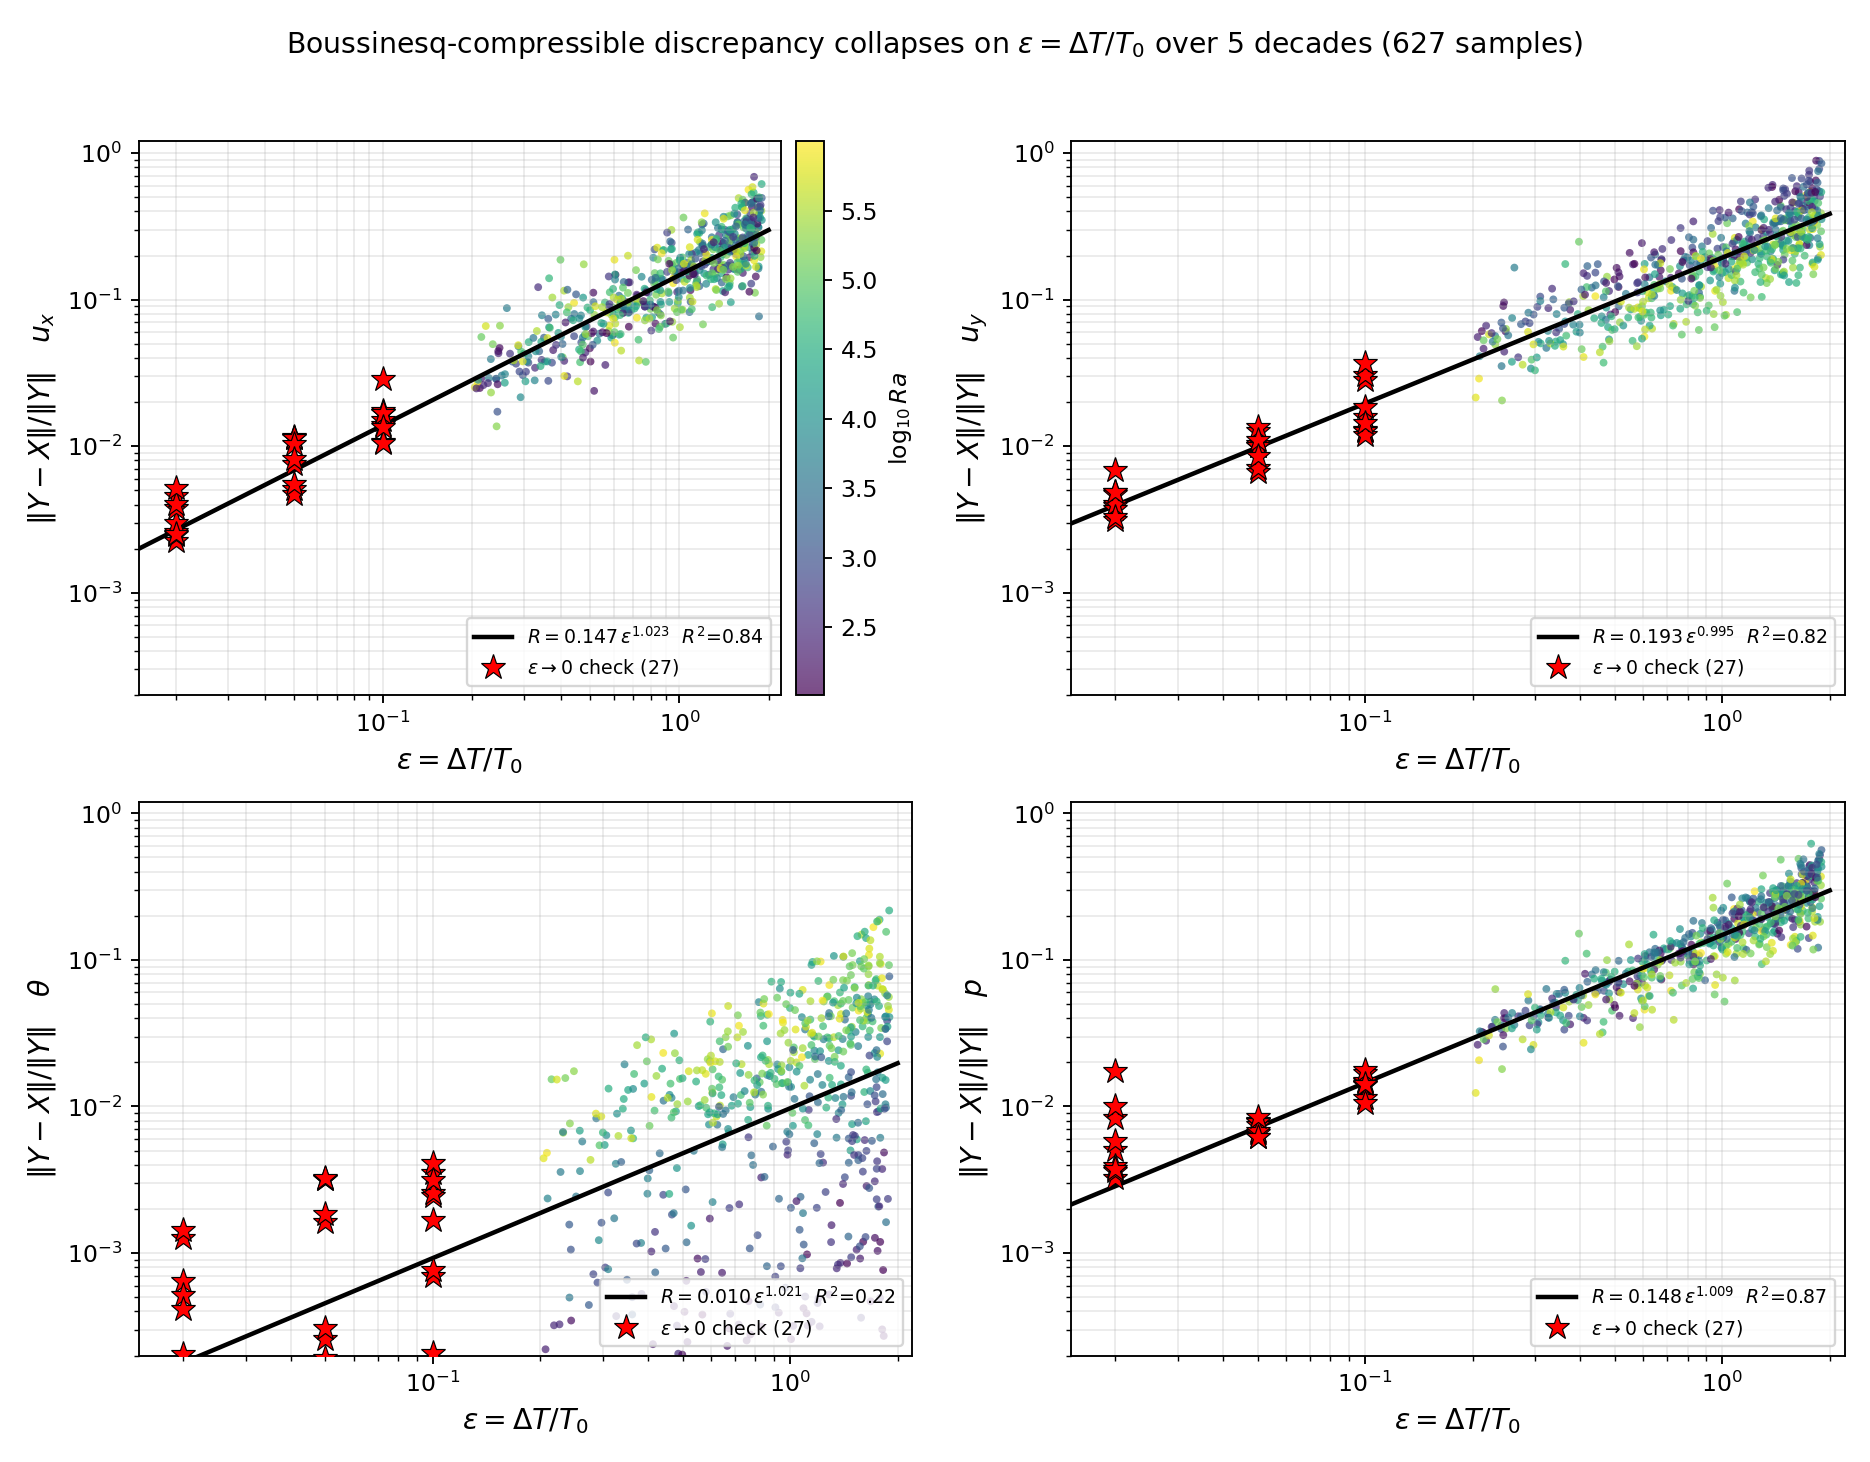
\includegraphics[width=0.95\textwidth]{fig1_law.png}
\caption{The Boussinesq--compressible discrepancy collapses on
$\varepsilon=\Delta T/T_0$ over two decades. Points: 600 random-boundary-condition samples,
coloured by $\log_{10}Ra$; stars: the 27 independent small-$\varepsilon$ checks. Lines: the
power-law fits of Table~\ref{tab:law}.}
\label{fig:law}
\end{figure}

\paragraph{The exponent is window-averaged, and the curvature is real.} The fit above uses the full
two decades, including the 27 check points at $\varepsilon\le0.1$ where $R$ is closest to its
linear limit. Fitting only $\varepsilon\ge0.8$ gives
$p=1.23\pm0.08/1.25\pm0.08/1.21\pm0.34/1.32\pm0.06$, and fitting each of the 20 paired
configurations separately over $\varepsilon\in[0.4,1.9]$ gives a median
$p=1.31/1.17/1.21/1.45$ (median $R^2=0.98$, \path{code/audit_v2.py}). That is the signature of
$R=A\varepsilon(1+\kappa\varepsilon)$ rather than of an exact power: a power law fitted to a curved
function over a window that excludes small $\varepsilon$ returns $p\approx1+\kappa\langle
\varepsilon\rangle$. The quadratic fit $R=a\varepsilon+c\varepsilon^2+b$ gives $c>0$ in all four
channels ($u_x$: $+0.0513\pm0.0133$, $3.9\sigma$; $u_y$: $+0.0695$; $\theta$: $+0.0060$; $p$:
$+0.0539$) with $\kappa=c/a=0.70/0.83/0.42/0.73$. We therefore state the law as \textbf{first order
in $\varepsilon$}, $R=A\varepsilon(1+O(\varepsilon))$, quote $p=1.02$ as the number a wide-window
fit returns, and note that the $\varepsilon^2$ curvature is independently recovered by the network
(Sec.~\ref{sec:prior}, $\beta=0.23$--$0.42$) and by the mode expansion (Sec.~\ref{sec:theory},
$\varepsilon^1+\varepsilon^2$ carry 99.0\% of the correction energy).

\begin{table}[htbp]
\centering
\small
\caption{Two-parameter refinement, $R=A\varepsilon^pRa^q$. The $Ra$ trend for $u_y$ and $\theta$
reproduces in the 2:1 geometry.}
\label{tab:two-param}
\begin{tabular}{@{}lcc@{}}
\toprule
channel & unit cavity ($n=600$) $p$ / $q$ / $R^2$ & aspect 2:1 ($n=104$) $p$ / $q$ / $R^2$\\
\midrule
$u_x$ & $1.081$ / $+0.003\pm0.006$ / $0.74$ & $1.071$ / $-0.143\pm0.019$ / $0.71$\\
$u_y$ & $1.016$ / $-0.083\pm0.005$ / $0.77$ & $1.146$ / $-0.077\pm0.019$ / $0.69$\\
$\theta$ & $1.120$ / $+0.514\pm0.015$ / $0.72$ & $0.989$ / $+0.447\pm0.045$ / $0.55$\\
$p$ & $1.127$ / $-0.029\pm0.005$ / $0.83$ & $1.057$ / $-0.154\pm0.017$ / $0.74$\\
\bottomrule
\end{tabular}
\end{table}

\begin{itemize}
\item $\varepsilon$-scaling is geometry-independent; the prefactor $A$ is not ($0.147\to0.175$ for
$u_x$, $0.148\to0.222$ for $p$, $0.193\to0.175$ for $u_y$, $0.010\to0.008$ for $\theta$).
\item Boundary-condition families barely matter \emph{inside this family}: 134 wall-mode families,
133 free dummies. Adding them to the $\varepsilon$-only fit raises the adjusted $R^2$ by 2.3 pp
($p$), 2.9 pp ($u_y$), 3.3 pp ($u_x$) and 8.5 pp ($\theta$)---the $\varepsilon$-scaling is not an
artefact of which wall modes were drawn (\path{code/audit_numbers.py}).
\item The $\theta$ channel needs one extra, cheaply available parameter, the advection strength of
the base flow $\chi=\|\bm u\|\|\nabla\theta\|/\|\theta\|$:
$R_\theta=\varepsilon(-0.0037+0.226\chi)$, $R^2$ $0.185\to\mathbf{0.778}$ (Spearman 0.902), i.e.\
$R_\theta\approx0.23\varepsilon\chi$. For $u_x/u_y/p$ adding $\chi$ does nothing. A single-input
form of the same statement, $R_\theta/\varepsilon=c\hat u^a$, is calibrated on two independent
generators in Sec.~\ref{sec:public} and carries the same information with $R^2=0.90$.
\item A pressure-channel preprocessing bug had to be fixed first (Sec.~\ref{sec:pressure}).
\end{itemize}
\subsection{A pressure-channel artefact, and why it mattered}
\label{sec:pressure}

Pairing the two members' \emph{raw} pressures mixes units: the compressible raw pressure carries a
hydrostatic ramp $12\times$ larger than its dynamic part, and the two weak forms use opposite
pressure sign conventions. Before the fix the per-sample median of $|X_p|/|Y_p|$ was $0.065$ and
that of $\cos(X_p,Y_p)$ was $-0.105$, and the $p$-channel ``law'' was a constant
($R_p\approx1.0$). Applying the recipe used by the public data set---subtract the mean, remove a
least-squares linear-in-$y$ fit, flip the sign of the Boussinesq member---gives $0.960$ and
$\cos=+0.991$ under the same median convention, against $0.929$ and $+0.986$ for the public
training set, i.e.\ we now match their pairing to within 3\% (\path{code/audit_v2.py}). The
channel then obeys the same law as the velocities ($A=0.148$, $p=1.009$). All $p$-channel numbers
reported here are post-fix.

\subsection{The $\varepsilon$-blind ceiling, measured exactly}
\label{sec:floor}

Within a configuration $X$ is identical for all $\varepsilon$, so an $\varepsilon$-blind model must
emit one field $F$ for every $\varepsilon$ it is applied at. Two reference protocols are exact
rather than fitted: (A) train at the one $\varepsilon$ a published data set offers (here
$\varepsilon=1.2$) and apply it everywhere, error $\|Y(\varepsilon)-Y(1.2)\|/\|Y(\varepsilon)\|$;
(B) the single field that best serves the whole range, the $\varepsilon$-mean of $Y$. (B) is a
least-squares compromise over the $\varepsilon$-range, \textbf{not a per-$\varepsilon$ lower
bound}---a field tuned to $\varepsilon=0.8$ gives $0.067$ at $\varepsilon=0.4$, better than (B)'s
$0.170$ there, and below $\varepsilon\approx0.8$ doing nothing beats both. Median over 20
configurations, channels $u_x/u_y/\theta/p$:

\begin{table}[htbp]
\centering
\footnotesize
\setlength{\tabcolsep}{4pt}
\caption{The exact $\varepsilon$-blind floor. Protocol (A) is what a single-$\varepsilon$ public
data set forces; protocol (B) is the best single field over the whole range. Entries are medians
over 20 configurations, ordered $u_x/u_y/\theta/p$.}
\label{tab:floor}
\begin{tabular}{@{}c p{4.5cm}p{4.5cm}p{4.5cm}@{}}
\toprule
$\varepsilon$ & do nothing ($\hat Y=X$) & (A) train at $\varepsilon=1.2$ only & (B)
$\varepsilon$-mean field\\
\midrule
0.4 & 0.060/0.098/0.009/0.061 & 0.143/0.219/0.021/0.146 & 0.170/0.244/0.023/0.177\\
0.8 & 0.127/0.203/0.019/0.129 & 0.078/0.118/0.011/0.082 & 0.108/0.143/0.013/0.126\\
1.2 & 0.211/0.328/0.030/0.220 & 0/0/0/0 & 0.035/0.036/0.003/0.051\\
1.6 & 0.322/0.481/0.044/0.347 & 0.112/0.151/0.014/0.131 & 0.079/0.123/0.012/0.085\\
1.9 & 0.472/0.616/0.058/0.547 & 0.251/0.304/0.031/0.346 & 0.225/0.286/0.028/0.281\\
\bottomrule
\end{tabular}
\end{table}

\begin{figure}[htbp]
\centering
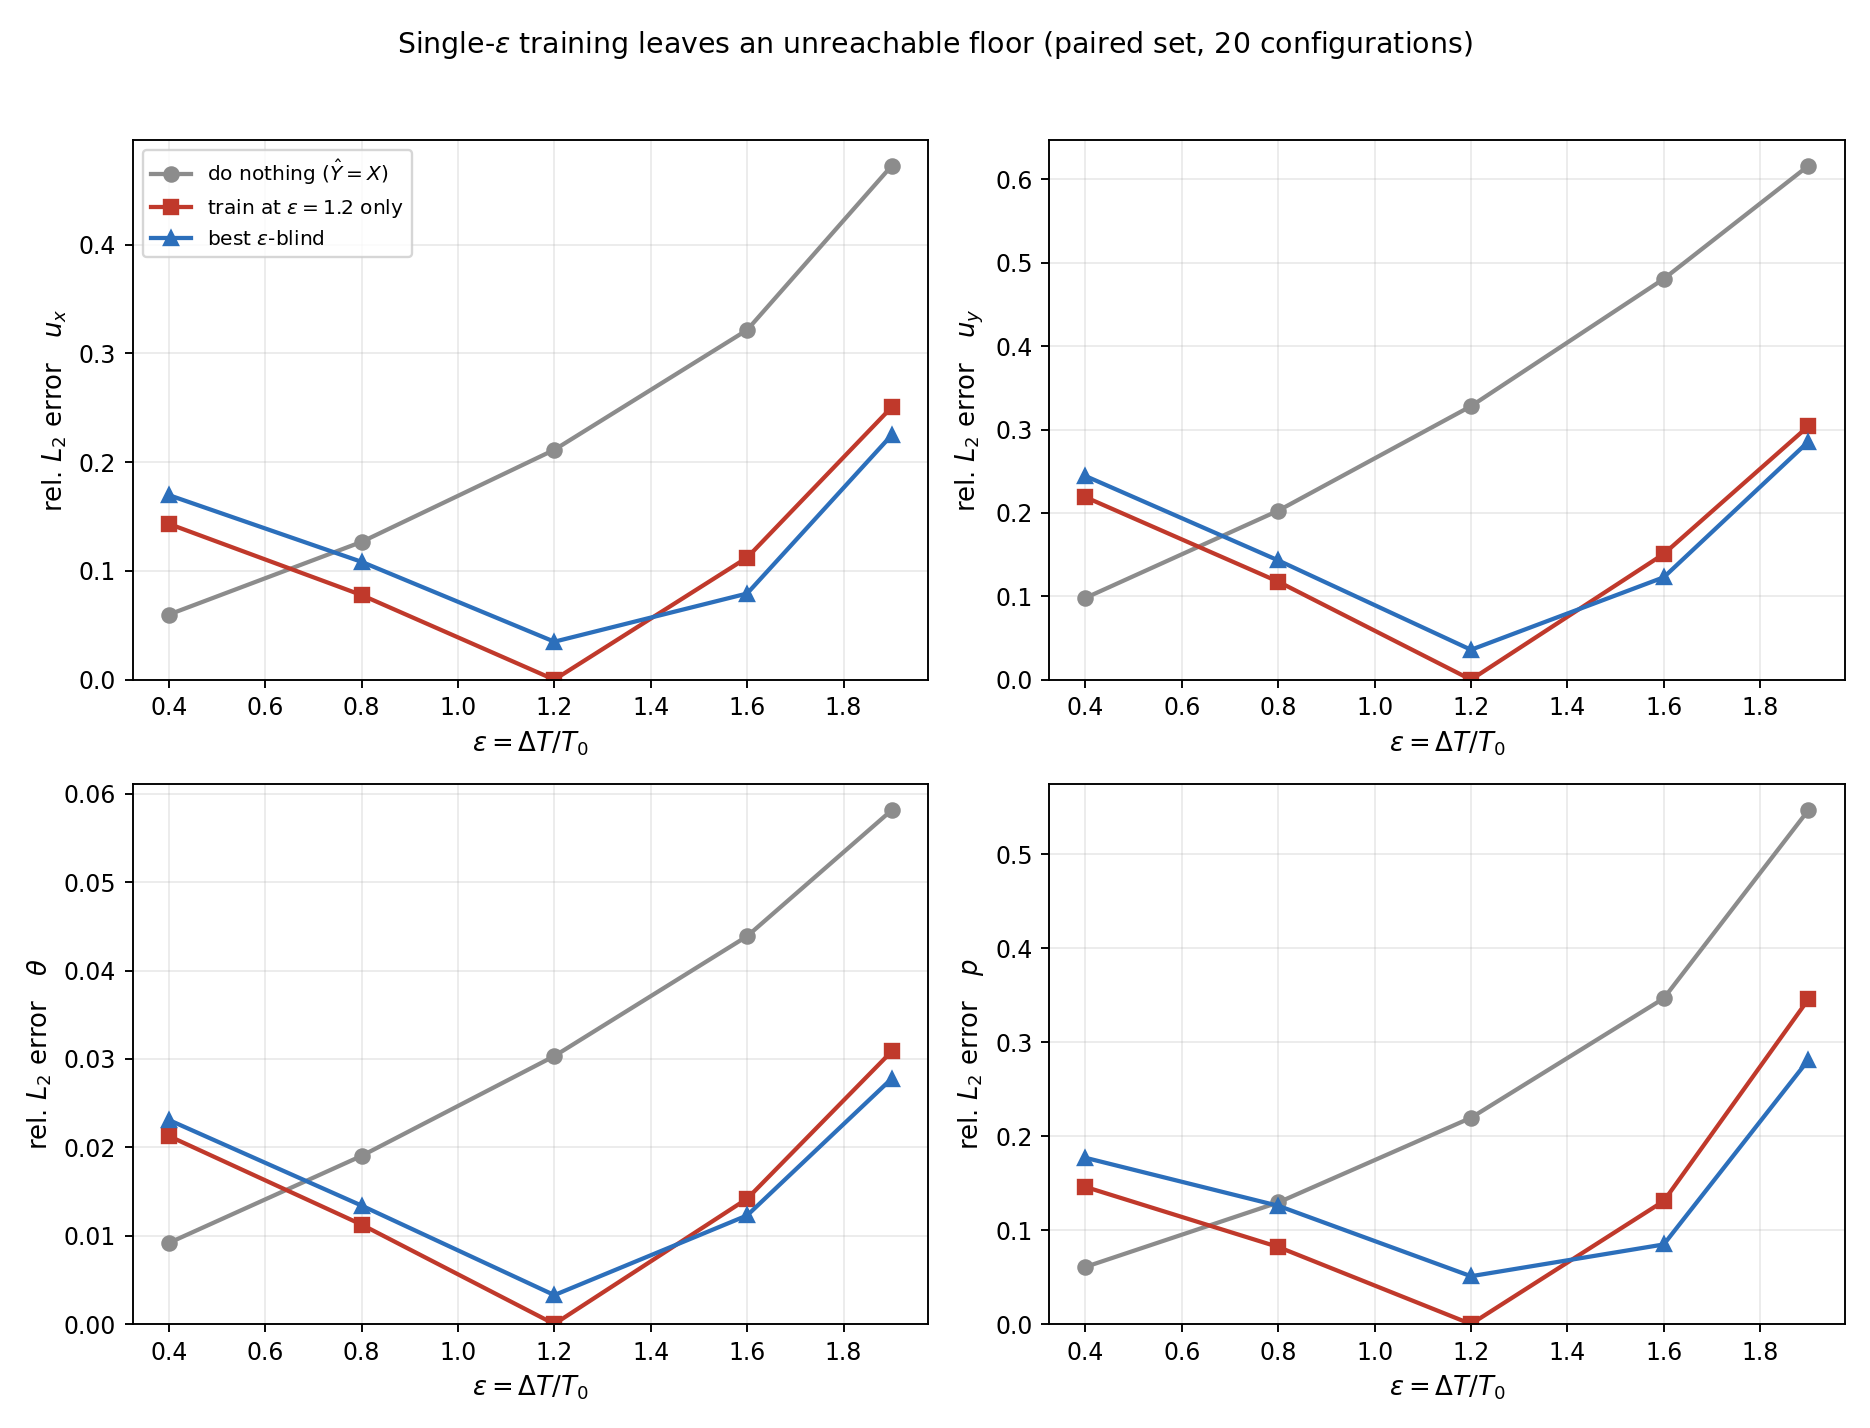
\includegraphics[width=0.95\textwidth]{fig2_floor.png}
\caption{Single-$\varepsilon$ training leaves an unreachable floor. Curves show ``do nothing'',
training at $\varepsilon=1.2$ only, and the best $\varepsilon$-blind field, for the 20 paired
configurations.}
\label{fig:floor}
\end{figure}

Protocol (A) is what a single-$\varepsilon$ public data set forces: 25\% ($u_x$), 30\% ($u_y$) and
35\% ($p$) error at $\varepsilon=1.9$, 8\% ($u_x$) already at $\varepsilon=0.8$, and---the point
for practice---at $\varepsilon=0.4$--$0.8$ ``do nothing'' is \emph{better} than it. Protocol (B),
the best an $\varepsilon$-blind model could possibly do over the range, still leaves
$22.5/28.6/28.1\%$ at $\varepsilon=1.9$. The whole effect is one line of arithmetic, and the paired
set measures it exactly (\path{code/exp_paired_final.py}; the diagonal is identically zero
because the same $\varepsilon$ is the same solution):

\begin{table}[htbp]
\centering
\small
\caption{Exact transfer error $R(u_x)$ when a field computed at one $\varepsilon$ (columns) is
applied at another (rows).}
\label{tab:transfer-matrix}
\begin{tabular}{@{}lccccc@{}}
\toprule
$R(u_x)$ applied at $\downarrow$ / taken from $\to$ & 0.4 & 0.8 & 1.2 & 1.6 & 1.9\\
\midrule
$\varepsilon=0.4$ & 0 & 0.067 & 0.143 & 0.235 & 0.353\\
$\varepsilon=0.8$ & 0.068 & 0 & 0.078 & 0.183 & 0.305\\
$\varepsilon=1.2$ & 0.149 & 0.081 & 0 & 0.110 & 0.243\\
$\varepsilon=1.6$ & 0.265 & 0.199 & 0.112 & 0 & 0.140\\
$\varepsilon=1.9$ & 0.402 & 0.328 & 0.251 & 0.142 & 0\\
\bottomrule
\end{tabular}
\end{table}

The error is set by the distance in $\varepsilon$ and by nothing else---which is precisely the
quantity $\varepsilon P(X)$ puts back into the model.

\subsection{Network baselines: the correction is information, not capacity}
\label{sec:baselines}

Table~\ref{tab:baselines} reports a U-Net of width 32, 200 epochs, mean of three seeds, identical
protocol for all columns (largest standard deviation over every cell: 0.0051).

\begin{table}[htbp]
\centering
\footnotesize
\setlength{\tabcolsep}{4pt}
\caption{U-Net ablation. A sees only the four Boussinesq fields; B also receives $\varepsilon$ as a
constant input channel. ``Energy recovered by B'' is $1-(R_B/R_{\mathrm{do\ nothing}})^2$.}
\label{tab:baselines}
\begin{tabular}{@{}p{4.2cm}cccccc@{}}
\toprule
split & channel & A (no $\varepsilon$) & B ($\varepsilon$ input) & gain & do nothing &
energy recovered by B\\
\midrule
extrapolation ($n=218$) & $u_x$ & 0.2289 & \textbf{0.1508} & $1.52\times$ & 0.3018 & 75\%\\
 & $u_y$ & 0.2733 & \textbf{0.1725} & $1.58\times$ & 0.3731 & 79\%\\
 & $\theta$ & 0.0406 & \textbf{0.0255} & $1.59\times$ & 0.0556 & 79\%\\
 & $p$ & 0.2689 & \textbf{0.1791} & $1.50\times$ & 0.3320 & 71\%\\
interpolation ($n=200$) & $u_x$ & 0.1530 & \textbf{0.0673} & $2.27\times$ & 0.2203 & 91\%\\
 & $u_y$ & 0.1796 & \textbf{0.0714} & $2.52\times$ & 0.2683 & 93\%\\
 & $\theta$ & 0.0261 & \textbf{0.0097} & $2.69\times$ & 0.0381 & 94\%\\
 & $p$ & 0.1792 & \textbf{0.0667} & $2.69\times$ & 0.2386 & 92\%\\
\bottomrule
\end{tabular}
\end{table}

Model A's error (0.2289) and the best possible $\varepsilon$-blind model on the paired set at
$\varepsilon=1.9$ (0.2249, Sec.~\ref{sec:floor}) agree to within 2\% while being measured on two
different data sets: the ceiling is informational, not architectural. Shallow learners plateau in
the same place. A linear ridge regression and an RBF kernel ridge on the raw four-field
input---the same information the network gets---reach $u_x$ 0.2282 and 0.2222 in extrapolation, and
adding $\varepsilon$ as an extra column barely moves them (0.2188 and 0.2171, against 0.0937 for
the structured model), because neither can represent a product of an $\varepsilon$-scale with a
spatial field. A classical POD-ROM (44--52 modes, 99.9\% of the snapshot energy) whose coefficients
are regressed on $(\log_{10}Ra,\varepsilon)$ lands at 0.2937 with $\varepsilon$ and 0.3001 without,
i.e.\ at the level of doing nothing, and a purely linear surrogate that also sees the POD
coefficients of $X$ reaches only 0.2318. The plateau is not capacity---it is that the quantity to be
added is absent from the input (\path{code/exp_shallow.py}, \path{code/exp_pod.py}).
\subsection{The physics prior: $D=\varepsilon P(X)$}
\label{sec:prior}

Same backbone, only the output structure changes ($\varepsilon$ still read from a constant channel,
target still $D$):

\begin{table}[htbp]
\centering
\small
\setlength{\tabcolsep}{4pt}
\caption{Output-factorisation ablation. P1 multiplies $\varepsilon$ outside the network; P2 adds a
learned quadratic term. $\beta$ is learned per channel and is the same sign and order as the
$\varepsilon^2$ coefficient of the expansion.}
\label{tab:prior}
\begin{tabular}{@{}llccccc@{}}
\toprule
split & variant & $u_x$ & $u_y$ & $\theta$ & $p$ & learned $\beta$\\
\midrule
extrapolation & plain U-Net & 0.1508 & 0.1725 & 0.0255 & 0.1791 & ---\\
 & $D=\varepsilon P(X)$ & 0.0937 & 0.1060 & 0.0141 & 0.1126 & fixed 0\\
 & $D=(\varepsilon+\beta\varepsilon^2)P(X)$ & \textbf{0.0867} & \textbf{0.0951} &
 \textbf{0.0131} & \textbf{0.1007} & 0.418/0.321/0.343/0.338\\
interpolation & plain U-Net & 0.0673 & 0.0714 & 0.0097 & 0.0667 & ---\\
 & $D=\varepsilon P(X)$ & 0.0545 & 0.0524 & 0.0078 & 0.0454 & fixed 0\\
 & $D=(\varepsilon+\beta\varepsilon^2)P(X)$ & \textbf{0.0507} & \textbf{0.0488} &
 \textbf{0.0073} & \textbf{0.0410} & 0.286/0.232/0.252/0.265\\
\bottomrule
\end{tabular}
\end{table}

\begin{figure}[htbp]
\centering
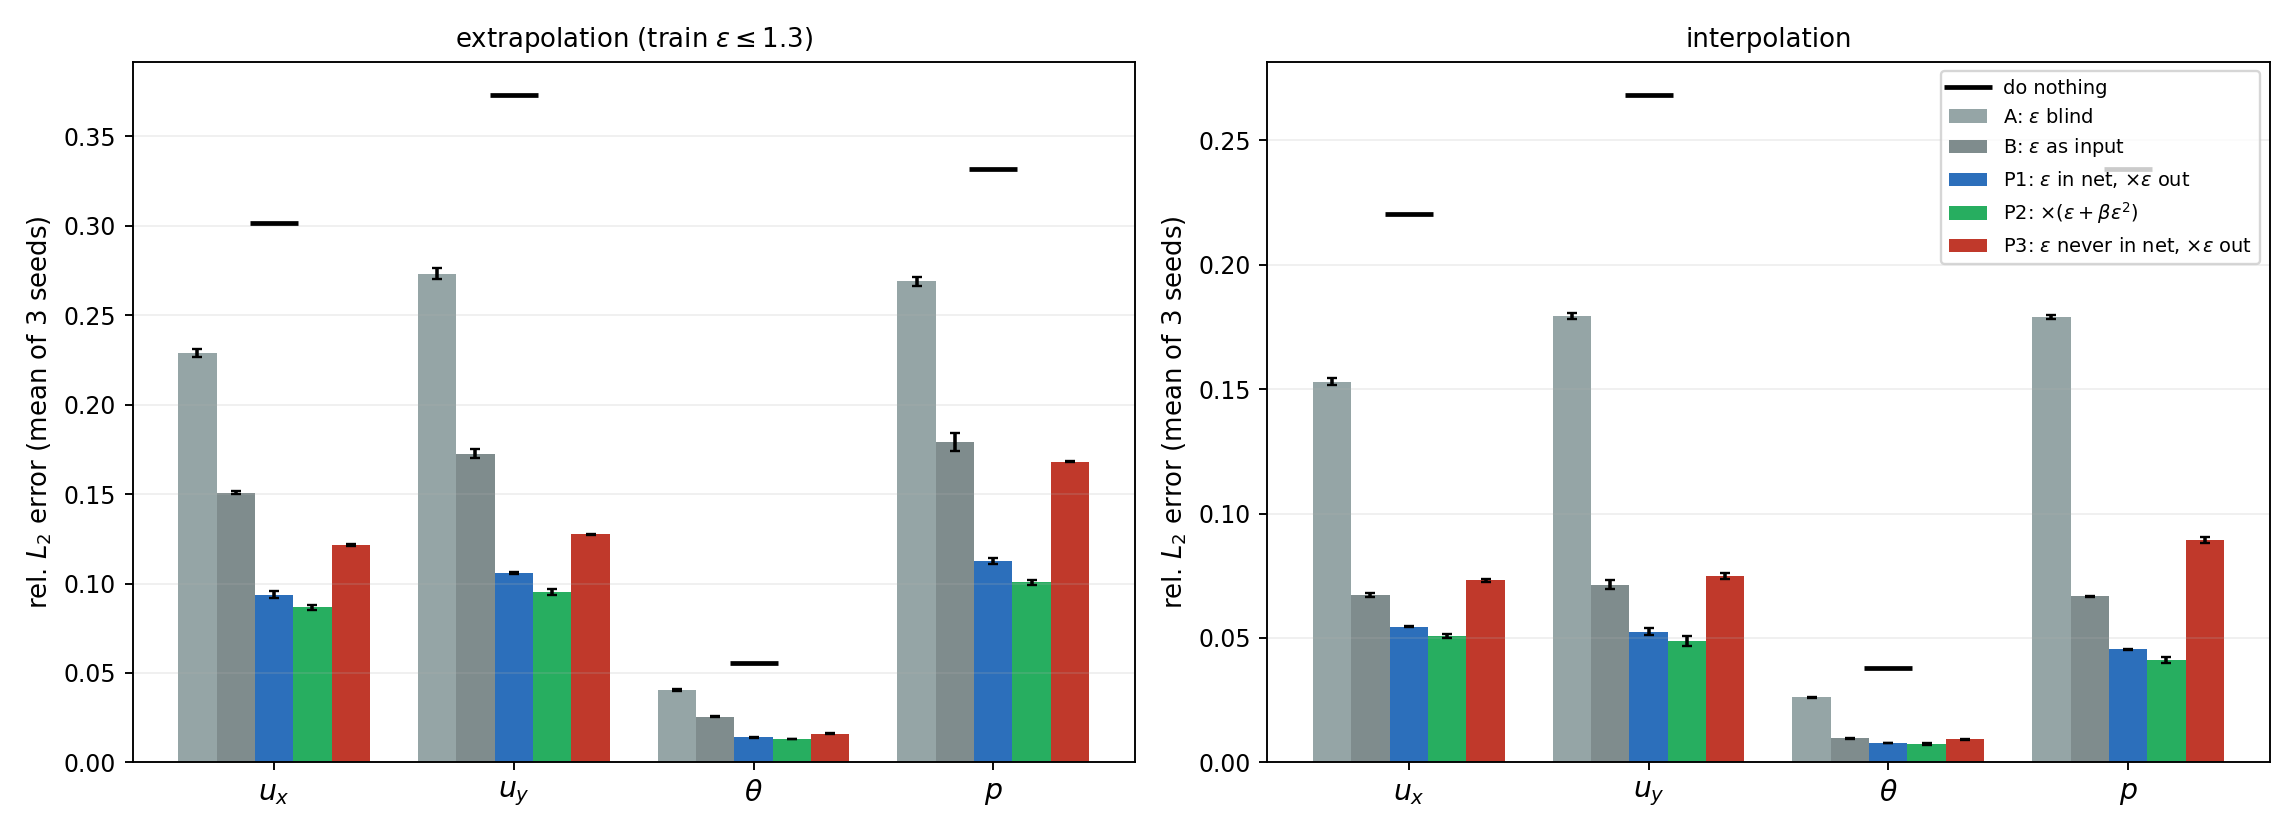
\includegraphics[width=0.98\textwidth]{fig3_prior.png}
\caption{The prior ablation for extrapolation (left) and interpolation (right). A: $\varepsilon$-blind.
B: $\varepsilon$ as input. P1: $\varepsilon$ in the network, multiplied outside. P2: learned
$(\varepsilon+\beta\varepsilon^2)$ factor. P3: $\varepsilon$ never enters the network.}
\label{fig:prior}
\end{figure}

Two things happen at once. In extrapolation the factorised output beats the plain one by
$\mathbf{1.61\times}$ ($u_x$) and $1.59$--$1.81\times$ in the other channels; the quadratic form adds
a further 7.6--10.6\% on top. And the network \emph{discovers} a positive curvature on its own,
$\beta=0.23$--$0.42$, the same sign and order as the $\varepsilon^2$ term of the expansion in
Sec.~\ref{sec:theory}---an independent check of the asymptotic expansion.

A Fourier neural operator (1.19\,M parameters) shows the same pattern against its
$\varepsilon$-blind version: $u_x$ $0.2287\to\mathbf{0.1334}$ with the prior and $\varepsilon$
multiplied back outside the network ($1.71\times$), statistically indistinguishable from an
explicit $\varepsilon$ input channel ($0.1334\pm0.0004$ against $0.1342\pm0.0008$). On $u_y$ and
$\theta$ the prior is in fact better (0.1387 against 0.1456; 0.0177 against 0.0191); only on $p$
does the $\varepsilon$ channel win (0.1536 against 0.1734). The prior's value is therefore not that
it beats an $\varepsilon$-aware model---it is that it matches one while needing no $\varepsilon$ in
the input (Secs.~\ref{sec:learning}, \ref{sec:transfer}).

\subsection{Data efficiency}
\label{sec:learning}

\begin{table}[htbp]
\centering
\footnotesize
\setlength{\tabcolsep}{4pt}
\caption{Learning curve on the fixed interpolation test set (200 samples), mean of three seeds.
Entries are $u_x/u_y/\theta/p$. P3 keeps $\varepsilon$ outside the network entirely.}
\label{tab:learning}
\begin{tabular}{@{}c p{6.0cm}p{6.0cm}@{}}
\toprule
$n$ & B: $\varepsilon$ as input & P3: predict $P(X)$, $\varepsilon$ outside\\
\midrule
0 (do nothing) & 0.2203/0.2683/0.0381/0.2386 & same\\
50 & 0.1831/0.1946/0.0269/0.1838 & \textbf{0.1308/0.1364/0.0195/0.1501}\\
100 & 0.1280/0.1422/0.0199/0.1348 & \textbf{0.0990/0.1022/0.0136/0.1150}\\
200 & 0.0974/0.1070/0.0147/0.0998 & \textbf{0.0827/0.0866/0.0114}/0.1005\\
400 & \textbf{0.0674/0.0714}/0.0097/\textbf{0.0672} & 0.0735/0.0743/0.0093/0.0896\\
\bottomrule
\end{tabular}
\end{table}

\begin{figure}[htbp]
\centering
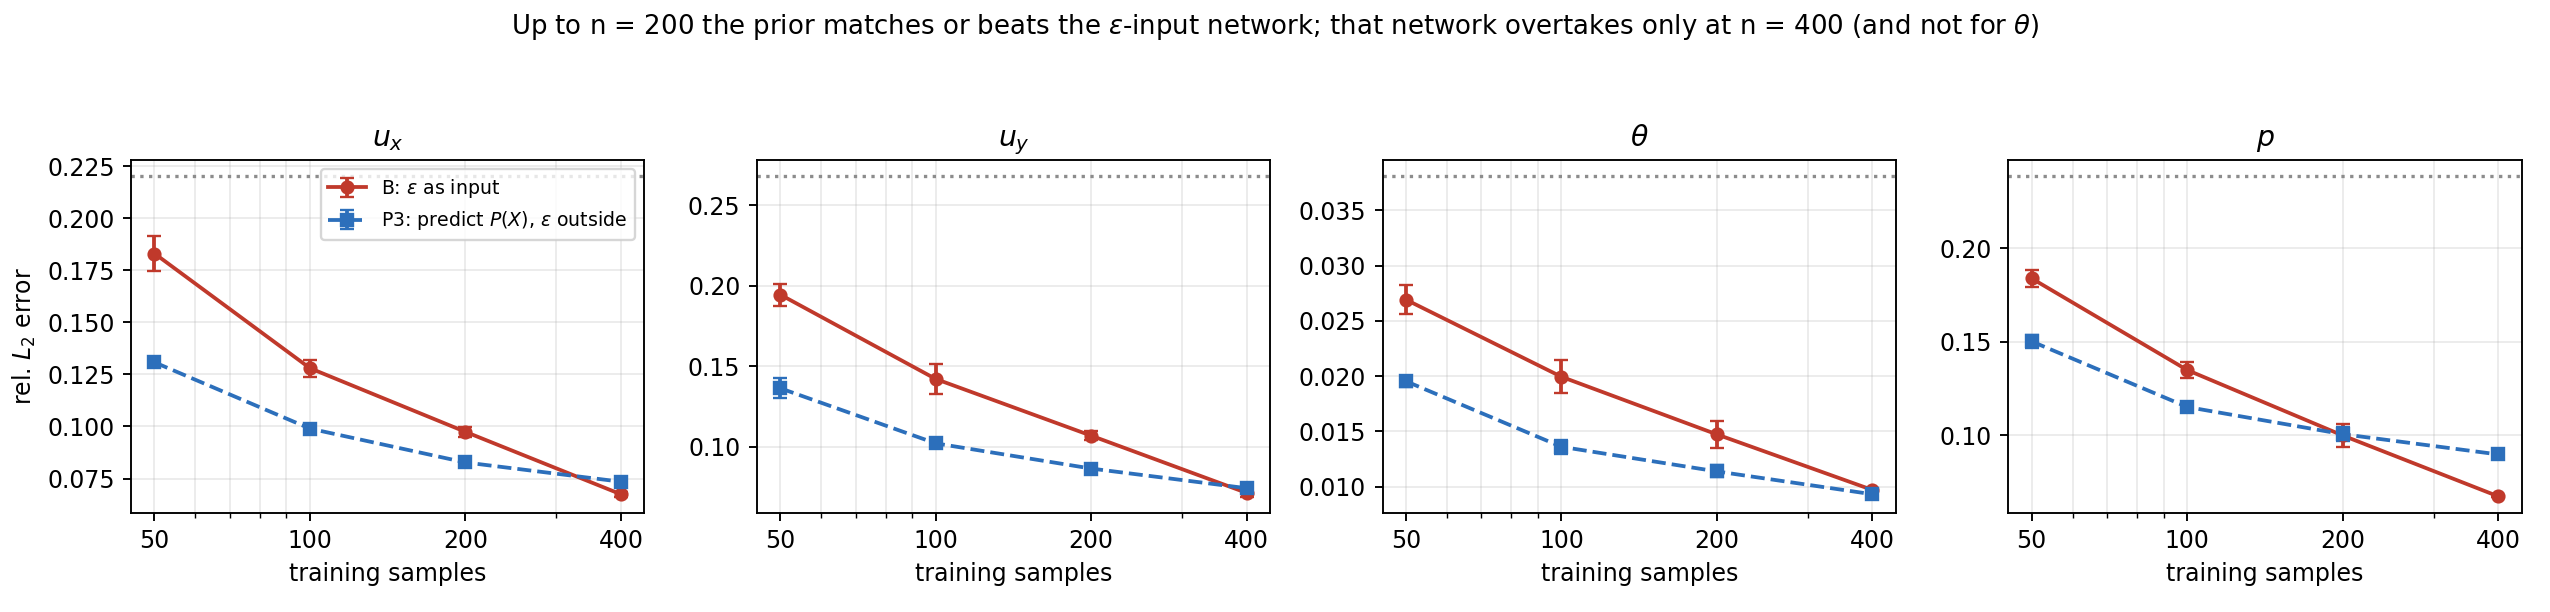
\includegraphics[width=0.98\textwidth]{fig4_learning.png}
\caption{Learning curves. Up to $n=200$ the prior matches or beats the $\varepsilon$-input network;
the latter overtakes only at $n=400$, and not for $\theta$.}
\label{fig:learning}
\end{figure}

The naive expectation---that a structured model trades in-distribution accuracy for
extrapolation---is wrong at small $n$. At $n=50$ the prior is $1.4\times$ better than the
$\varepsilon$-input network ($u_x$ 0.1308 against 0.1831, a $9\sigma$ separation across three seeds),
and it is still ahead at $n=200$ in $u_x$ ($7.3\sigma$), $u_y$ ($7.6\sigma$) and $\theta$
($3.6\sigma$), with $p$ already level ($0.13\sigma$) there. The crossover sits between $n=200$ and
400 in $u_x$ and $u_y$ (log-linear interpolation: $n\approx315$ and 360, i.e.\ near 300 in $u_x$),
essentially at $n=200$ in $p$, and $\theta$ never crosses---at $n=400$ it is still $2.5\sigma$
behind. Concretely, the prior at $n=200$ reaches what the $\varepsilon$-input network needs
$\approx270$ samples ($u_x$) and 290 ($u_y$) to reach. So the prior is two things at once: the
cheaper model when data is scarce, and---the point that matters for reuse---a model that needs no
$\varepsilon$ in its input, which is what makes a single-$\varepsilon$ data set reusable.

\subsection{External validation on an independent, published data set}
\label{sec:public}

\path{NurshatMenglik/NeuralConvection_2D_TrainTest} (v2; 4000 training pairs plus 200
in-distribution test pairs, CC BY 4.0), generated by another group with their own pipeline, at a
\textbf{single} $\varepsilon=1.2$, $Ra\in[10^2,3\cdot10^6]$ \citep{menglik2026neural}.

\paragraph{Conventions match.} Recomputing their published \path{relL2_*} columns as
$\|Y-X\|/\|X\|$ from the tensors reproduces them exactly (0.14233/0.13749/0.01356/0.19070 for
sample 0); their pressure amplitude ratio is 0.929 against 0.931 for our fixed pairing.

\paragraph{The law reproduces.} On the $\varepsilon=1.2$ slice:

\begin{table}[htbp]
\centering
\small
\caption{External validation at $\varepsilon=1.2$: public data against our own slice. Medians with
p10--p90 in parentheses.}
\label{tab:public}
\begin{tabular}{@{}lcc@{}}
\toprule
channel & public 4000 (median, p10--p90) & our data at $\varepsilon\in[1.1,1.3]$ ($n=64$)\\
\midrule
$u_x$ & 0.1797 (0.112--0.300) & 0.1839 (0.126--0.284)\\
$u_y$ & 0.2435 (0.141--0.403) & 0.2250 (0.150--0.395)\\
$\theta$ & 0.0228 (0.001--0.071) & 0.0232 (0.001--0.056)\\
$p$ & 0.1858 (0.117--0.246) & 0.1889 (0.128--0.262)\\
\bottomrule
\end{tabular}
\end{table}

\paragraph{Even the secondary trends reproduce.} The correlation of $R$ with $\log_{10}Ra$ is
$+0.133/-0.419/+0.647/-0.198$ on their $\varepsilon\equiv1.2$ data and
$+0.032/-0.511/+0.662/-0.263$ on our $\varepsilon\in[1.1,1.3]$ slice (64 samples,
$u_x/u_y/\theta/p$). The $\theta$ channel---the one whose scatter we explain next---has $r=+0.66$ on
ours and $+0.65$ on theirs, from independently generated data.

\paragraph{Five splits, four prefactors, one predictable pattern.} The release publishes three
further held-out splits generated by the same generator and the same solver commit
(\path{v6_freefall_20260921}, \path{raw_both_deramp} pressure convention; the OOD split
carries the later tag \path{v6_freefall_ood_20260925}): \path{test_in_distribution} (200
random-wall pairs), \path{test_ood} (200 random-wall pairs whose vertical-wall Fourier dials lie
outside the training range) and \path{test_legacy} (200 pairs of the classical cavity: constant
hot and cold side walls, adiabatic top and bottom). We had already downloaded
\path{train_legacy}, 5000 classical-cavity pairs. Recomputing all of \path{relL2_u_x},
\path{relL2_u_y}, \path{relL2_T}, \path{relL2_p} for \textbf{every sample of all five
splits (38\,400 values: 9600 samples $\times$ 4 channels)} under our conventions reproduces the
published numbers to within $1.2\times10^{-7}$ (float32 round-off;
\path{code/verify_conventions.py}), so nothing below is a convention artefact. At the fixed
$\varepsilon=1.2$ the medians of $R=\|Y-X\|/\|Y\|$ are:

\begin{table}[htbp]
\centering
\small
\caption{Median relative correction on all five public splits, at $\varepsilon\equiv1.2$.}
\label{tab:splits}
\begin{tabular}{@{}lccccc@{}}
\toprule
split & $n$ & $u_x$ & $u_y$ & $\theta$ & $p$\\
\midrule
train (random walls) & 4000 & 0.1797 & 0.2435 & 0.0228 & 0.1858\\
test\_in\_distribution & 200 & 0.1822 & 0.2388 & 0.0220 & 0.1863\\
test\_ood (harder wall dials) & 200 & 0.1567 & 0.2157 & 0.0214 & 0.1671\\
train\_legacy (classical cavity) & 5000 & 0.2988 & 0.3362 & 0.0926 & 0.1989\\
test\_legacy (classical cavity) & 200 & 0.2984 & 0.3390 & 0.0836 & 0.1983\\
\bottomrule
\end{tabular}
\end{table}

The exponent cannot be re-tested here---every split sits at one $\varepsilon$---but the prefactor is
put under pressure and it moves: by $1.66\times$ ($u_x$), $1.38\times$ ($u_y$), $4.05\times$
($\theta$) and $1.07\times$ ($p$) between the classical cavity and the random-wall families at the
same $\varepsilon$, and \path{train_legacy} and \path{test_legacy} agree to three digits in
$u_x$ and $p$ ($\theta$: 0.0926 vs 0.0836, 10\%), which is the internal consistency check for the
whole comparison. That is a statement about the flow, not a defect of the law, and the $\theta$
channel makes the mechanism explicit. Writing $\hat u=\max\|\bm u_X\|$, the peak speed of the
Boussinesq field (hence available to any surrogate):

\begin{table}[htbp]
\centering
\small
\caption{The $\theta$-channel prefactor is the flow strength: $R_\theta/\varepsilon=c\hat u^a$ on
six data sets from two independent generators.}
\label{tab:uhat}
\begin{tabular}{@{}lccc@{}}
\toprule
data set & $n$ & $R_\theta/\varepsilon=c\hat u^a$ & $R^2$\\
\midrule
ours, random walls, $Pr=0.71$ & 600 & $a=1.864\pm0.026$, $c=0.544$ & 0.90\\
public train, random walls & 4000 & $a=1.902\pm0.010$, $c=0.602$ & 0.91\\
public test\_in\_distribution & 200 & $a=1.977\pm0.041$, $c=0.691$ & 0.92\\
public test\_ood & 200 & $a=1.931\pm0.041$, $c=0.561$ & 0.92\\
public train\_legacy, classical cavity & 5000 & $a=2.360\pm0.002$, $c=2.063$ & \textbf{0.995}\\
public test\_legacy, classical cavity & 200 & $a=2.368\pm0.011$, $c=2.095$ & \textbf{0.996}\\
\bottomrule
\end{tabular}
\end{table}

\begin{figure}[htbp]
\centering
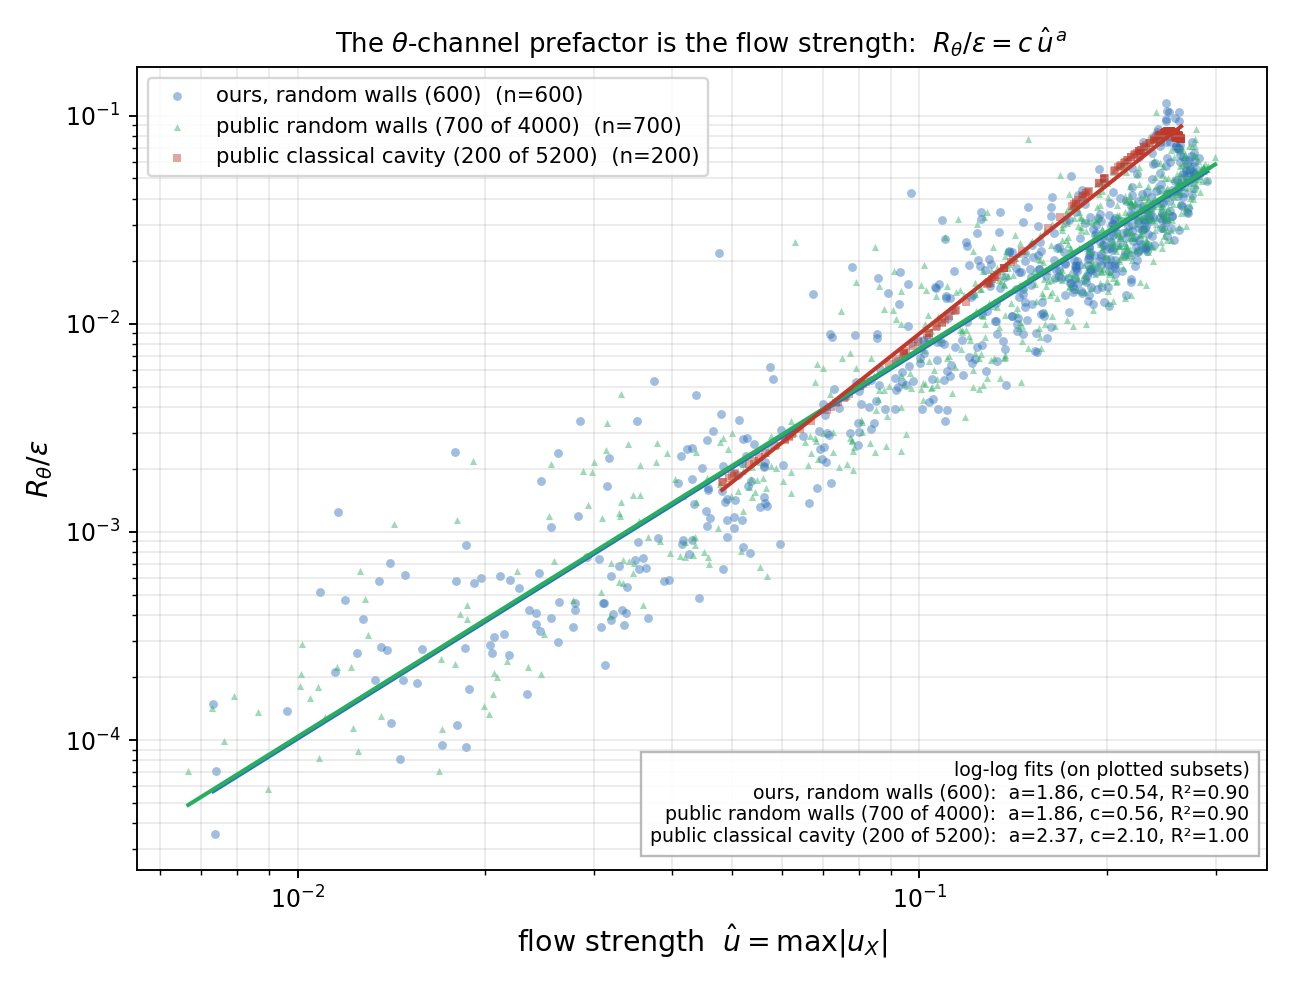
\includegraphics[width=0.78\textwidth]{fig7_theta_flow.png}
\caption{The $\theta$-channel prefactor collapses on the peak Boussinesq speed $\hat u$ across two
independent generators and two boundary-condition families.}
\label{fig:theta}
\end{figure}

Two independent groups, two independent generators, six data sets: the random-wall families all give
$c=0.54$--$0.69$, the classical cavity---whose flow is a single strong circulation with $\hat u$
41\% above the public random-wall median and 56\% above ours---gives $c=2.06$--$2.10$
(\path{code/exp_uhat_law.py}). The same reading explains the residual scatter in $u_x/u_y/p$ in
Sec.~\ref{sec:law}: $A$ is a functional of the flow, and the flow is in the input.
\subsection{Cross-data-set transfer: the payoff, and its boundary}
\label{sec:transfer}

Two public single-$\varepsilon$ data sets are available: 4000 random-wall pairs (our
boundary-condition family) and 5000 classical-cavity pairs (a different one). Both sit at
$\varepsilon\equiv1.2$. We train the same U-Net on each---once with the plain output (target $D$),
once with the prior (target $D/\varepsilon$, and $\varepsilon$ multiplied back outside the
network)---and apply the result to \textbf{our own 600 samples with no retraining}, at
$\varepsilon$ from 0.2 to 1.9, values the training data never contained.

\begin{table}[htbp]
\centering
\footnotesize
\setlength{\tabcolsep}{4pt}
\caption{Transfer from a single-$\varepsilon$ public data set to our own
$\varepsilon\in[0.2,1.9]$ samples. Entries are $u_x/u_y/\theta/p$.}
\label{tab:transfer}
\begin{tabular}{@{}p{5.0cm}p{1.0cm}p{4.4cm}p{4.4cm}@{}}
\toprule
trained on & model & $\varepsilon>1.3$, $n=218$ & full $\varepsilon$, $n=200$\\
\midrule
do nothing & $\hat Y=X$ & 0.3018/0.3731/0.0556/0.3320 & 0.2203/0.2683/0.0381/0.2386\\
public 4000, random walls, $\varepsilon\equiv1.2$ & plain &
0.1443/0.1730/0.0226/0.1838 & 0.1199/0.1441/0.0189/0.1435\\
public 4000, random walls, $\varepsilon\equiv1.2$ & \textbf{prior} &
\textbf{0.0932/0.1085/0.0119/0.1322} & \textbf{0.0657/0.0769/0.0077/0.0891}\\
our own 382 training samples & prior & 0.1250/0.1321/0.0170/0.1719 &
0.0791/0.0811/0.0103/0.0947\\
public 5000, classical cavity, $\varepsilon\equiv1.2$ & plain &
0.2919/0.3711/0.0490/0.3192 & 0.2444/0.3612/0.0484/0.3217\\
public 5000, classical cavity, $\varepsilon\equiv1.2$ & prior &
0.3092/0.4730/0.0561/0.3280 & 0.2281/0.3498/0.0422/0.2584\\
\bottomrule
\end{tabular}
\end{table}

\begin{figure}[htbp]
\centering
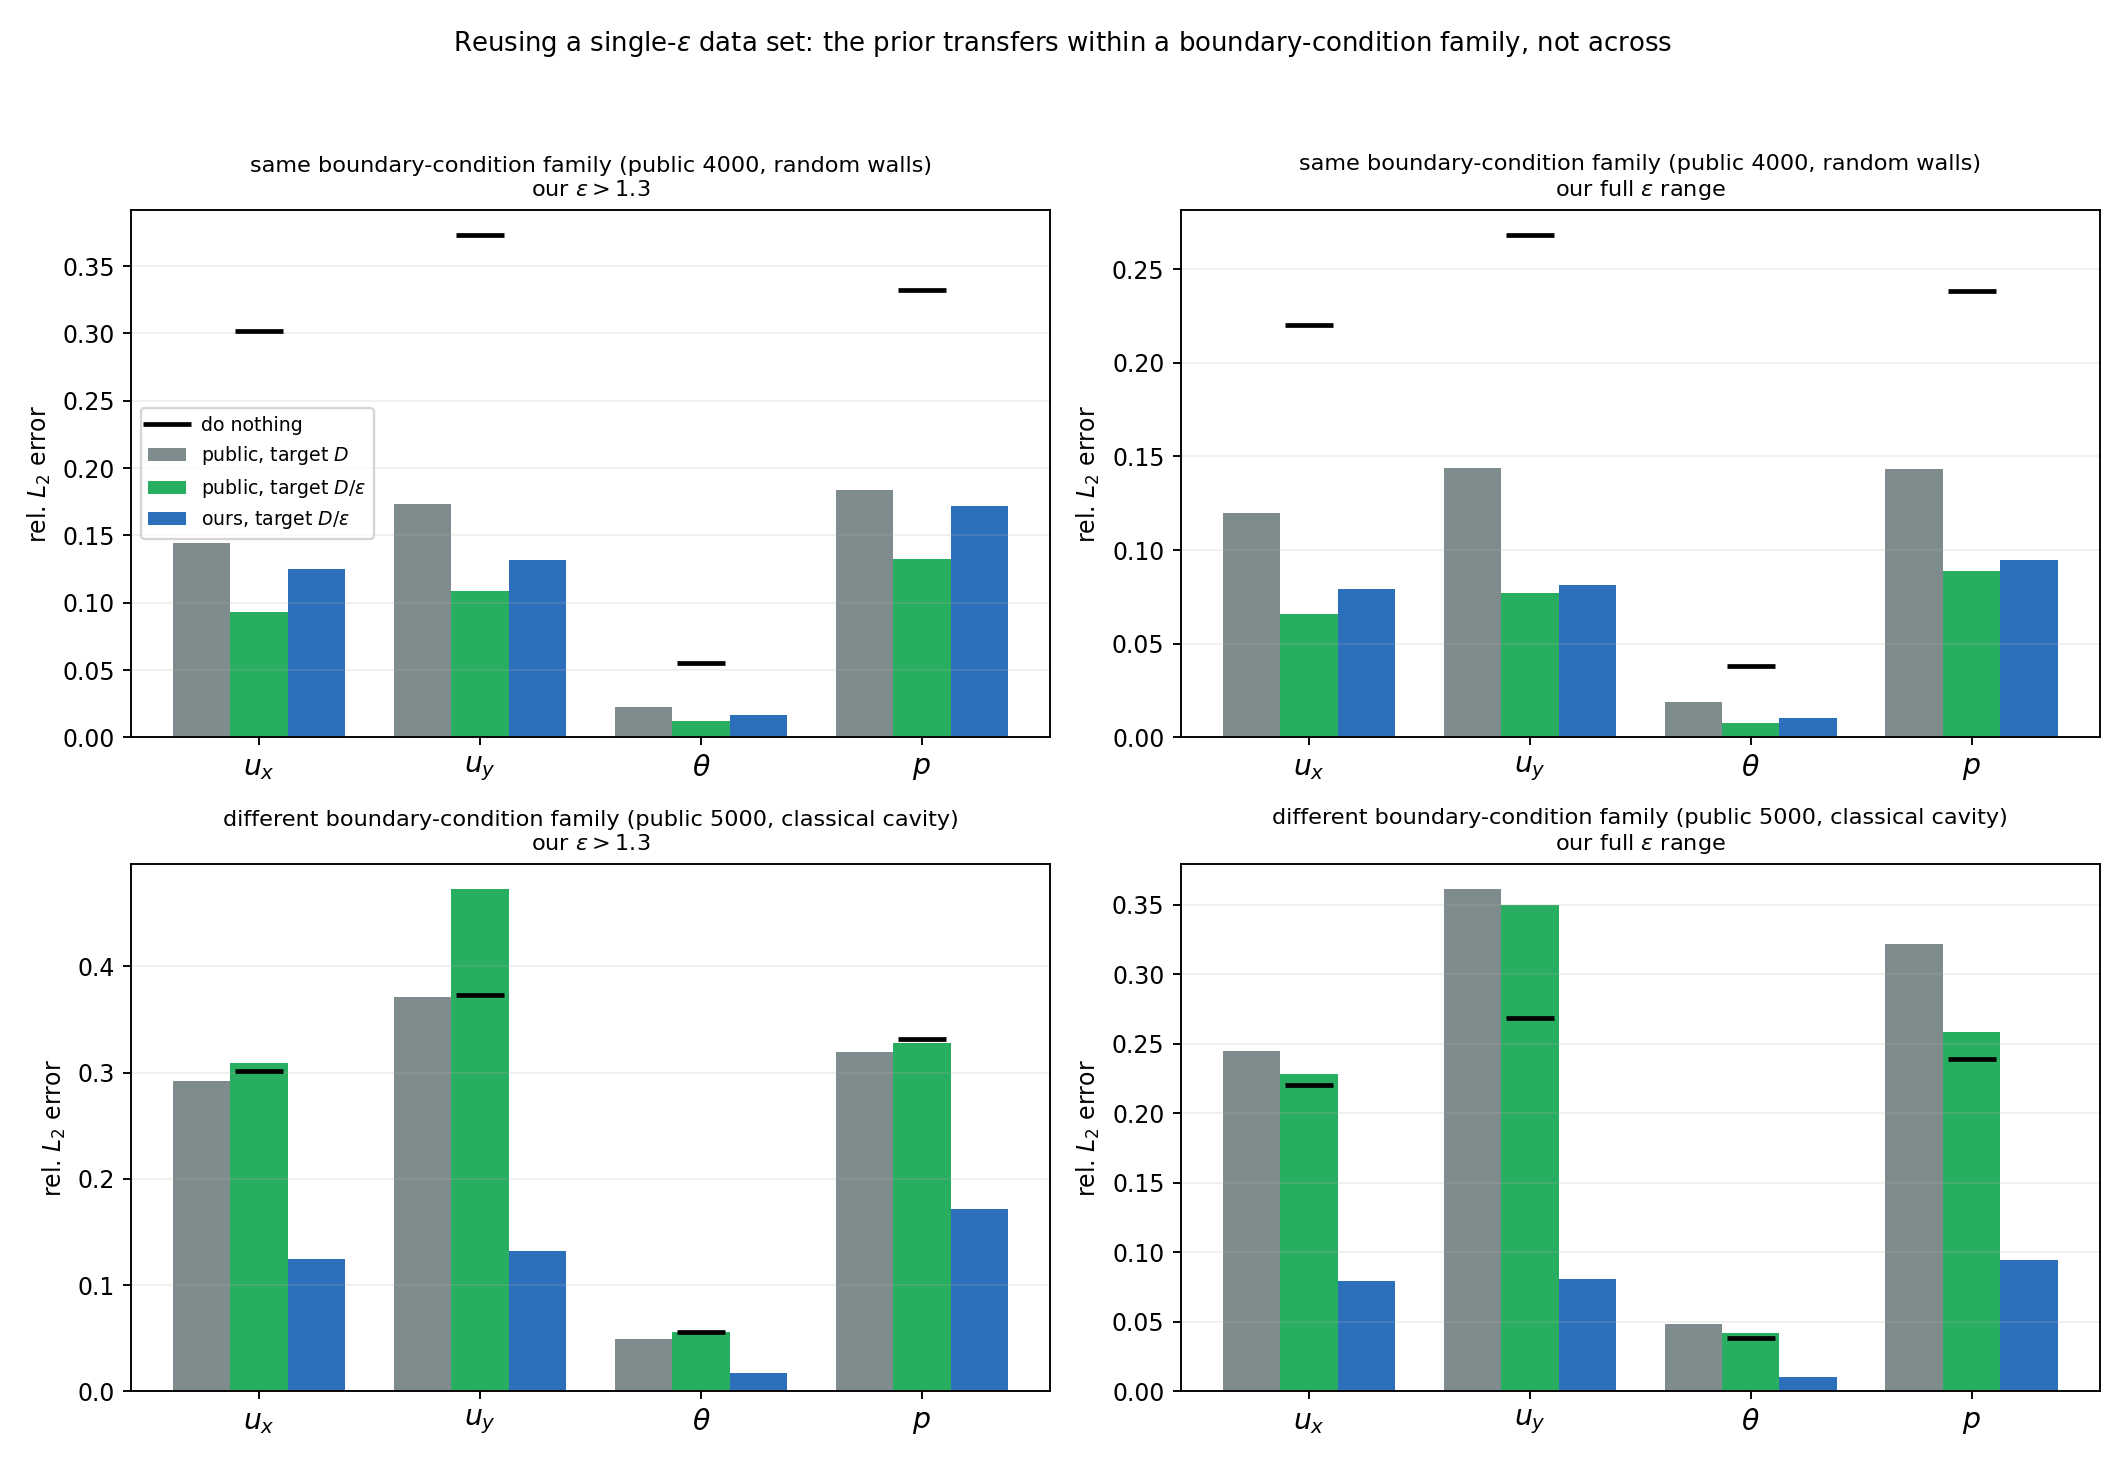
\includegraphics[width=0.9\textwidth]{fig6_transfer.png}
\caption{Reusing a single-$\varepsilon$ data set. Within the boundary-condition family the prior
transfers and beats the plain model; across families it fails, and can be worse than doing
nothing.}
\label{fig:transfer}
\end{figure}

Three readings, in order of how much they matter for practice.

\begin{itemize}
\item \textbf{Within the family, the prior is what makes a single-$\varepsilon$ data set reusable.}
The identical architecture, budget and data give 0.1443 ($u_x$) with the plain output and 0.0932
with the prior---a factor 1.55---and $3.2\times$ better than doing nothing, on $\varepsilon$ the
data never contained. It is even better than the same prior trained on our own 382 samples
(0.1250), because it sees ten times more configurations. This is the concrete content of ``the
$\varepsilon$ dependence need not be in the data''.
\item \textbf{The prior also fixes the failure mode of the plain model.} The plain model's error at
unseen $\varepsilon$ is largest where the training $\varepsilon$ is furthest away (its correction
is a fixed field, Sec.~\ref{sec:floor}), whereas the prior's error stays proportional to how wrong
$P$ is, uniformly in $\varepsilon$.
\item \textbf{Across boundary-condition families the same trick fails, and the prior makes it
worse.} Trained on the classical cavity, the plain model lands at 0.2919 against a floor of
0.3018---it learned almost nothing transferable---and the prior model is \emph{worse} than the
plain one (0.3092 at $\varepsilon>1.3$): it confidently multiplies a $P$ learnt on the wrong flow by
an $\varepsilon$ that grows to 1.9. This is exactly what Sec.~\ref{sec:public} predicts, and it is
the same number: $A$ is a functional of the flow, the classical cavity's flow has $\hat u$ 41\%
above the random-wall median, and a surrogate trained on that family predicts the wrong $A$.
Reusing published data therefore requires the boundary-condition family to be represented; the law
tells you in advance which reuse will work (\path{code/exp_public_transfer.py},
\path{code/exp_public_legacy_transfer.py}).
\end{itemize}

\subsection{A second geometry (aspect ratio 2:1, 104 samples)}
\label{sec:aspect}

Same generator, same $Ra$ and $\varepsilon$ ranges, cavity twice as wide. The $\varepsilon$
exponent is unchanged ($p=1.09/1.16/0.93/1.08$ for $u_x/u_y/\theta/p$, $0.7\sigma$, $1.8\sigma$,
$0.3\sigma$ and $0.7\sigma$ away from the unit-square values), while the prefactor moves
($A=0.175/0.175/0.008/0.222$ versus $0.147/0.193/0.010/0.148$). The Rayleigh trend is stronger for
$u_x$ and $p$ here ($q=-0.14,-0.15$ vs $0.00,-0.03$) and reproduces for $u_y$ and $\theta$.
\textbf{The $\varepsilon$-scaling is geometry-independent; calibration of $A$ is not}---which is
exactly why the surrogate takes $X$ as input rather than a table of $A$. Changing the fluid instead
($Pr$ $0.71\to4.38$) moves neither the exponent nor the prefactor (Sec.~\ref{sec:water}).

\begin{figure}[htbp]
\centering
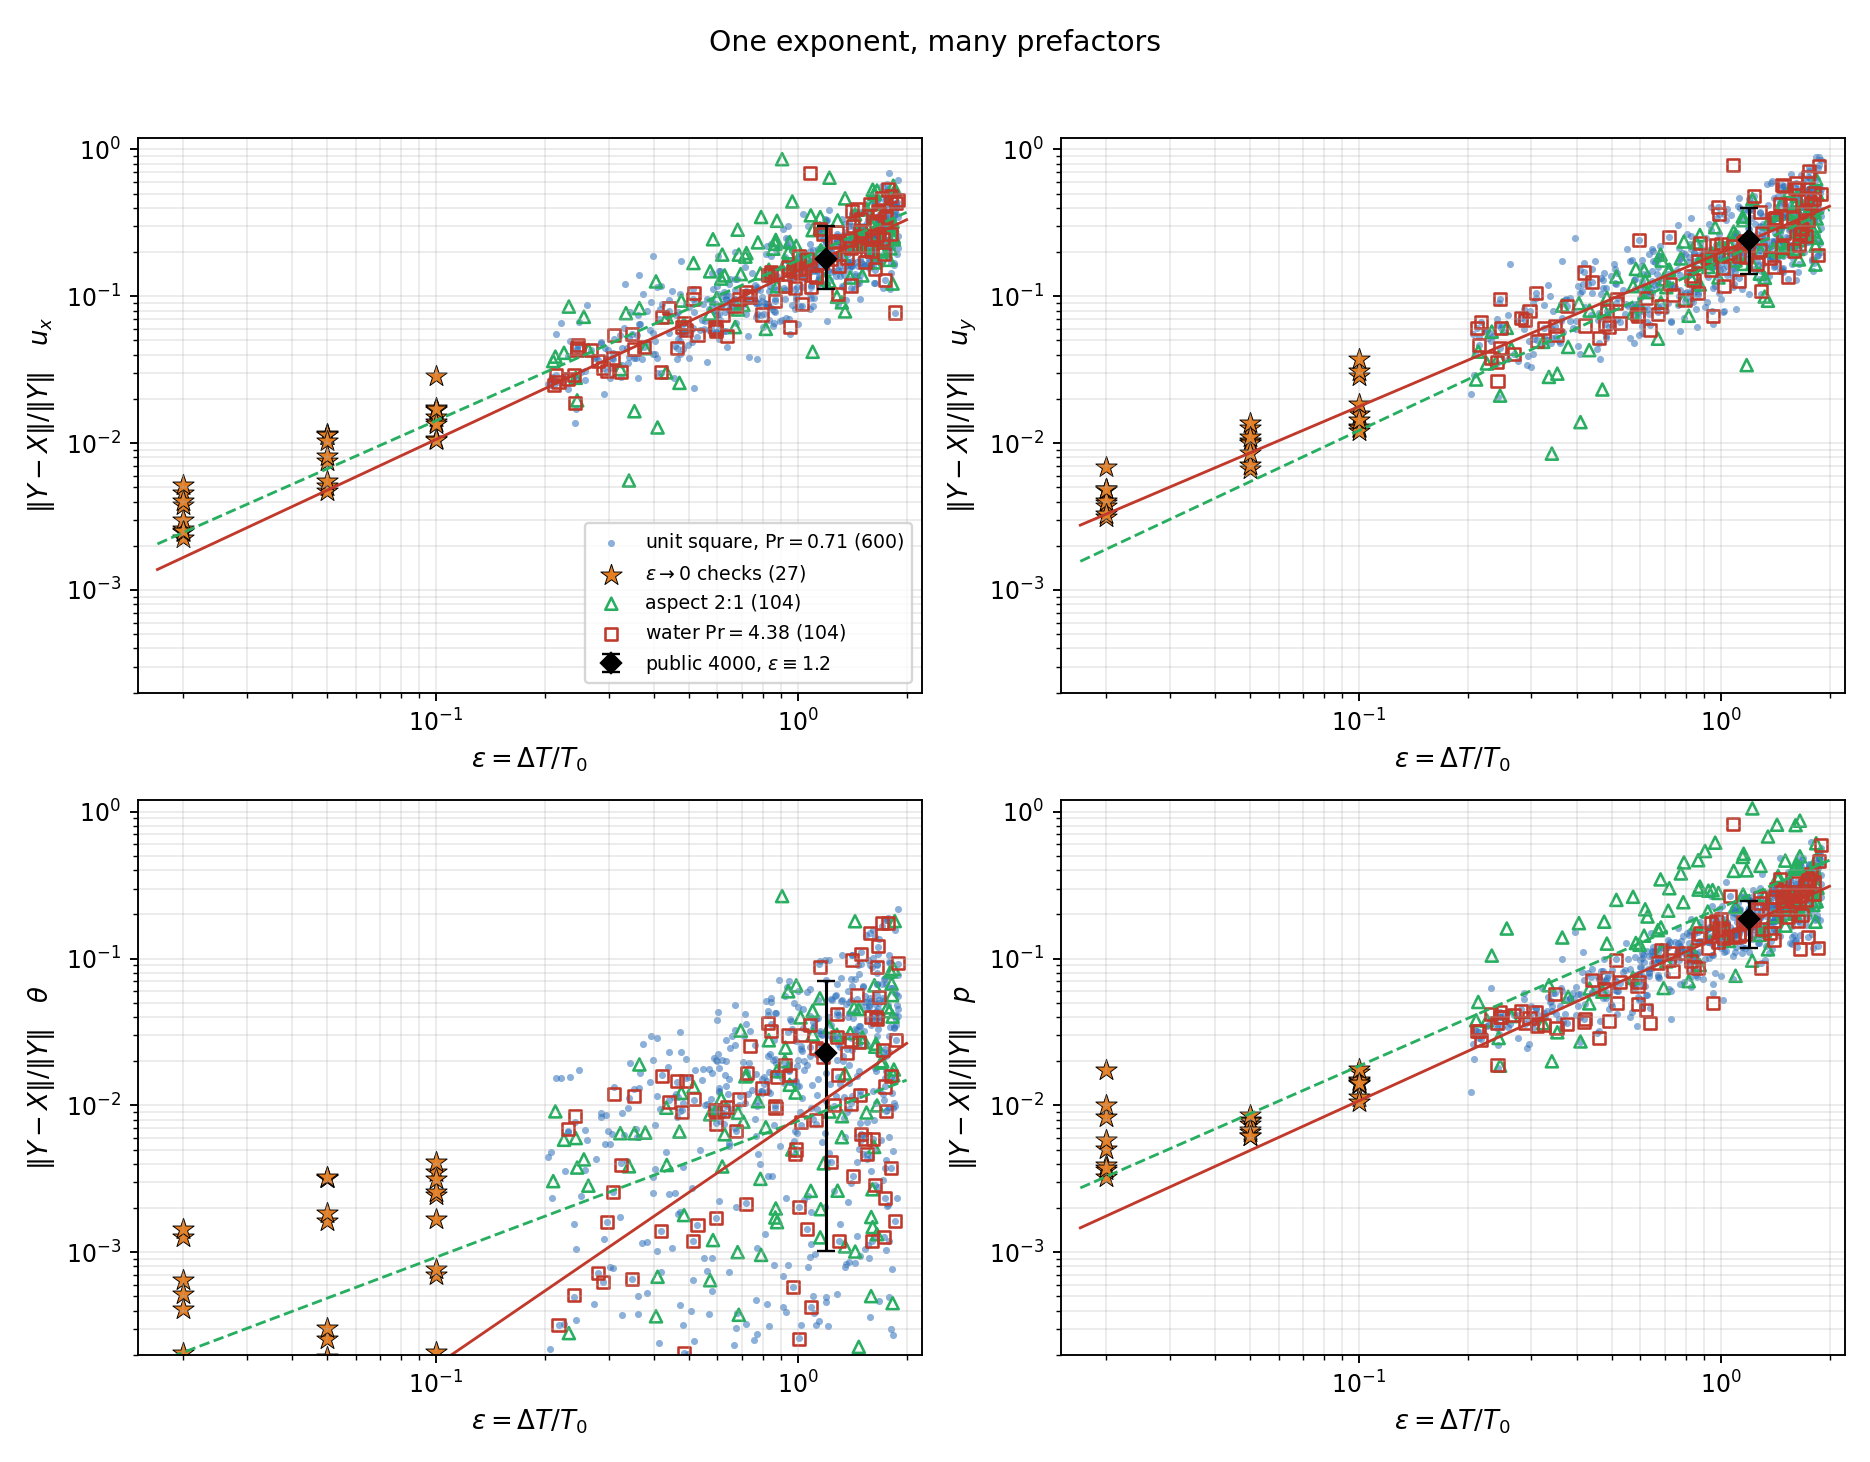
\includegraphics[width=0.95\textwidth]{fig5_law_axes.png}
\caption{One exponent, many prefactors: unit square ($Pr=0.71$), aspect 2:1, water
($Pr=4.38$), and the public data set at $\varepsilon=1.2$.}
\label{fig:axes}
\end{figure}

\subsection{Solver noise is not the source of the law}
\label{sec:noise}

\begin{itemize}
\item Convergence quality over 600 samples (compressible member): median relative change
$3.75\times10^{-6}$, p90 $1.09\times10^{-4}$, worst $7.04\times10^{-4}$.
\item Dropping the 65 samples with relative change $>10^{-4}$ changes the $u_x$ fit from
$0.1809\varepsilon-0.0212$ to $0.1813\varepsilon-0.0221$---unchanged.
\item Re-running the 10 worst samples with \path{steady_tol} tightened from $10^{-6}$ to
$10^{-8}$ leaves the solution \textbf{bit-identical} ($|\Delta Y|/|Y|=0$). The reason is
structural: the compressible march terminates on the zero-iteration guard, not on
\path{steady_tol}, so the residual reported is the fixed-point residual of the discrete solution,
not unfinished iteration.
\end{itemize}

\subsection{Cost and speed-up}
\label{sec:cost}

\begin{table}[htbp]
\centering
\small
\caption{Wall-clock cost on one RTX 4060 Laptop, $64^2$ mesh, eight-way parallel solver.}
\label{tab:cost}
\begin{tabular}{@{}lcccc@{}}
\toprule
 & median & mean & p90 & max\\
\midrule
paired solve, 600 samples & 33.9\,s & 38.0\,s & 59.9\,s & 510\,s\\
paired solve, paired set & 55.8\,s & 67.7\,s & 136\,s & 202\,s\\
surrogate, GPU, batch 1 & 6.3\,ms & & &\\
surrogate, GPU, batch 256 & 0.49\,ms/sample & & &\\
surrogate, CPU, 1 thread & 14.0\,ms & & &\\
\bottomrule
\end{tabular}
\end{table}

The resulting factors are $\mathbf{5.4\times10^3}$ per sample and $\mathbf{6.9\times10^4}$ in
batches.

\subsection{A third fluid: $Pr=4.38$ (water)}
\label{sec:water}

$Pr$ and $\varepsilon$ do not mix. $Pr$ enters the coefficients of both members
($Re^{-1}=(Pr/Ra)^{1/2}$) and hence the Boussinesq solution $X$, but the $\varepsilon$-expansion of
Sec.~\ref{sec:theory} never multiplies the two. The prediction is therefore sharp and asymmetric:
the exponent must not move, while the prefactor may, because $X$ itself has changed.

We generated 104 further pairs at $Pr=4.38$ (water at $20^\circ$C) that are \textbf{bit-identical to
the first 104 samples of the main batch in every other respect}: same seed stream, hence the same
wall-temperature Fourier draws, the same $Ra$ and the same $\varepsilon$. The two families are
therefore a strict paired experiment in which the fluid is the only difference (the Mach-number law
is unchanged, and $Ma$ is inert, Sec.~\ref{sec:axis}).

\begin{table}[htbp]
\centering
\footnotesize
\setlength{\tabcolsep}{3pt}
\caption{The fluid axis: 104 strictly paired air/water configurations. The exponent is unchanged;
the prefactor moves by less than 5\% on the paired comparison.}
\label{tab:water}
\begin{tabular}{@{}p{4.2cm}cccccc@{}}
\toprule
 & $\varepsilon$ & $Ra$ & $u_x$ & $u_y$ & $\theta$ & $p$\\
\midrule
$Pr=0.71$, air (unit square) & 0.2--1.9 & $10^2$--$10^6$ &
0.1468 & 0.1934 & 0.0097 & 0.1482\\
$Pr=4.38$, water (104 paired) & 0.21--1.89 & $1.1\cdot10^2$--$8.9\cdot10^5$ &
0.1496 & 0.1985 & 0.0082 & 0.1426\\
$Pr=4.38$, $p$ & & & $1.150\pm0.054$ & $1.049\pm0.063$ & $1.686\pm0.238$ &
$1.124\pm0.054$\\
\bottomrule
\end{tabular}
\end{table}

\begin{figure}[htbp]
\centering
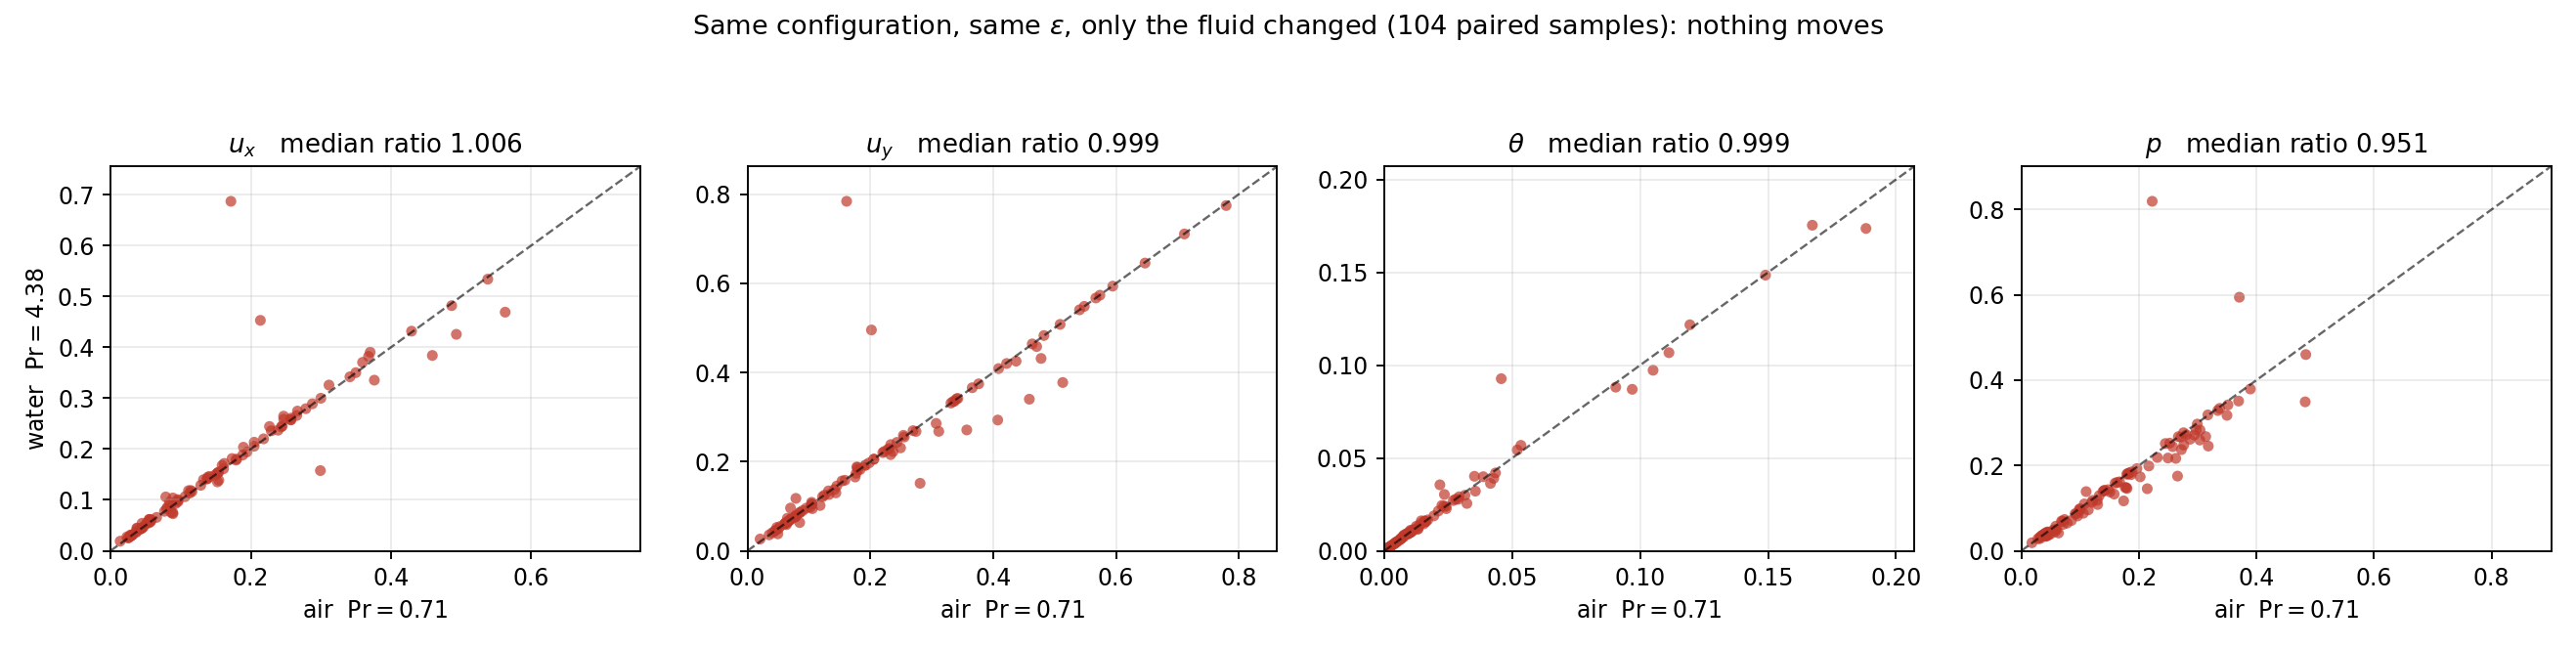
\includegraphics[width=0.96\textwidth]{fig8_water.png}
\caption{Same configuration, same $\varepsilon$, only the fluid changed: air ($Pr=0.71$) against
water ($Pr=4.38$), 104 paired samples.}
\label{fig:water}
\end{figure}

On the 104 matched configurations the paired ratios $R_{\mathrm{water}}/R_{\mathrm{air}}$ have
medians $\mathbf{1.006}$, $\mathbf{0.999}$, $\mathbf{0.999}$ and $\mathbf{0.951}$ ($u_x/u_y/\theta/p$; p10--p90
0.99--1.12, 0.90--1.03, 0.95--1.06, 0.82--1.00), and the paired exponents agree to three digits:
$1.150$ vs $1.157$, $1.049$ vs $1.047$, $1.686$ vs $1.668$, $1.124$ vs $1.109$. A 6.2-fold change
in Prandtl number---air to water---moves the Boussinesq--compressible discrepancy by less than 1\%
on the same configuration.

$Pr$ is therefore not a break-symmetry axis either, and the law's two ingredients separate cleanly:
$\varepsilon$ sets the exponent, the flow sets the prefactor, and the fluid does neither. Keeping
the strict pairing matters for the last digit---the unpaired fits give $\theta$ $0.0097\to0.0082$
(a 15\% move, the same direction as the 5\% paired move) and $u_x/u_y$ $+2$--3\%---which is the same
statement as Sec.~\ref{sec:aspect} (a geometry moves $A$) and Sec.~\ref{sec:public}
(boundary-condition families move it by up to $4\times$).
\section{Limitations}
\label{sec:limits}

\begin{enumerate}
\item \textbf{Two dimensions only.} A three-dimensional pair at $res=16$ costs $\ge23$\,min for the
Boussinesq member alone (1386\,s for 21 steady steps) and the compressible member was still
unfinished when a 30-minute wall-clock cap killed it (\path{code/run_3d_probe.sh},
\texttt{timeout 1800}); the historical $res=24$ probe at $\varepsilon=1.2$ never converged (Newton
backtracking to $dt=3.7\times10^{-4}$). A 3-D $\varepsilon$-sweep is out of reach on this machine
and we do not claim one.
\item \textbf{$Ma$ is inert here}, so the break-symmetry group is one-dimensional rather than two.
At larger $Ma$ this would have to be redone.
\item $\varepsilon<2$, imposed by the equation of state (the cold wall must stay positive).
\item The two-parameter fits of Sec.~\ref{sec:law} leave 26/23/28\% of the variance unexplained in
$u_x/u_y/\theta$ and 17\% in $p$; the $\hat u$ form of Sec.~\ref{sec:public} closes that gap for
$\theta$ and leaves the same residual flow-dependence in the other three channels.
\item The prefactor $A$ is configuration-dependent and must be learned: it moves with the geometry
(Sec.~\ref{sec:aspect}) and by $1.66\times$ ($u_x$) / $1.38\times$ ($u_y$) / $4.05\times$
($\theta$) / $1.07\times$ ($p$) between boundary-condition families of an independent data set
(Sec.~\ref{sec:public}), while it is insensitive to the fluid ($Pr$, Sec.~\ref{sec:water}).
\item The public data set and ours differ by 0.08\% in $Ra_{\mathrm{eff}}$ at $\varepsilon=1.2$
($1.2/1.095^2=1.000813$); their v2 release corrects this and the two now agree.
\end{enumerate}

\section{Conclusion}
\label{sec:conclusion}

We set out to build a surrogate for compressible natural convection and found that the object it has
to reproduce---the gap between the Boussinesq solution and the compressible one---is governed by a
single parameter in an exact and predictable way.

\begin{enumerate}
\item \textbf{One parameter.} In this non-dimensionalisation $Fr^2=\Delta T/T_0$ identically, so
the break-symmetry axis is $\varepsilon=\Delta T/T_0$ and nothing else; Mach-number effects are
$O(Ma^2)$ and are invisible at the values reached here.
\item \textbf{A clean law.} $R=\|Y-X\|/\|Y\|=A\varepsilon^p$ with
$p=1.023\pm0.018$, $0.995\pm0.019$, $1.024\pm0.077$, $1.009\pm0.015$ ($u_x,u_y,\theta,p$), an
intercept indistinguishable from zero, the exponent quoted over the full two-decade window (from
$\varepsilon=0.8$ upwards the same points give $1.23$--$1.32$, the $\varepsilon^2$ curvature of
Sec.~\ref{sec:law}), and a 134-family boundary-condition description (133 dummies) that adds only
2--3 pp of adjusted $R^2$ to the velocity and pressure channels. The exponent is
geometry-independent and fluid-independent; only the prefactor $A$ must be calibrated, which is why
the surrogate takes $X$ as input rather than a table of $A$.
\item \textbf{A reason.} The $\varepsilon$-expansion of the compressible member reproduces the
Boussinesq system at $O(1)$ and produces the correction through
$\nabla\cdot\bm u_1=\nabla\cdot(\theta_0\bm u_0)$ and the density-modulated inertia. The linearised
operator does not contain $\varepsilon$, so the correction factorises,
$D=\varepsilon P(X)+\varepsilon^2Q(X)+\dots$, with a shape that does not rotate. All five
consequences of the expansion are confirmed numerically.
\item \textbf{A design rule.} Predicting $P(X)$ and multiplying by $\varepsilon$ outside the
network---four lines of code---converts the law into a prior that (i) beats the plain architecture
by $1.61\times$ in extrapolation, (ii) lets the network discover the $\varepsilon^2$ term itself,
(iii) works the same way for a Fourier neural operator, and (iv) makes a public data set that exists
at a single temperature contrast reusable at others---0.093 ($u_x$) on $\varepsilon>1.3$ against
0.144 for the plain model and 0.302 for doing nothing---which is the difference between a surrogate
that must be retrained and one that can be applied. The scope of that reuse is set by
Sec.~\ref{sec:public}: it holds within a boundary-condition family and fails across one,
predictably.
\end{enumerate}

The honest limits are in Sec.~\ref{sec:limits}: two dimensions, $\varepsilon<2$, one-dimensional
break symmetry, and a prefactor whose two-parameter fits leave 26\% ($u_x$), 23\% ($u_y$) and 28\%
($\theta$) of the variance unexplained. None of them touch the claim that matters for practice,
which is that the $\varepsilon$ dependence is known in closed form and should not be left to the
network to discover from data.

\section{Reproducibility}
\label{sec:repro}

All scripts are in the \path{code/} directory of the project (Chinese-path Windows workspace,
executed in WSL2 with dolfinx 0.7.3 for the solver and PyTorch 2.10 for the surrogates); raw data,
logs and JSON results are under \path{~/nc_run/}.

\begin{table}[htbp]
\centering
\footnotesize
\setlength{\tabcolsep}{4pt}
\caption{Scripts and the results they produce.}
\label{tab:scripts}
\begin{tabular}{@{}>{\raggedright\arraybackslash}p{5.2cm}>{\raggedright\arraybackslash}p{10.4cm}@{}}
\toprule
script & what it produces\\
\midrule
\path{exp_eps_law.py} & the 627-sample law (Sec.~\ref{sec:law})\\
\path{repack_p_fixed.py} & the corrected pressure channel (Sec.~\ref{sec:pressure})\\
\path{exp_paired_final.py} & the $\varepsilon$-blind floor and shape invariance
(Sec.~\ref{sec:floor})\\
\path{exp_modes.py} & the $\varepsilon^k$ mode expansion (Sec.~\ref{sec:theory})\\
\path{exp_chi.py} & the $\chi$ explanation for $\theta$ (Sec.~\ref{sec:law})\\
\texttt{harness.py}, \path{exp_ml_final.py} & the unified surrogate ablation: A/B/P1/P2/P3,
three seeds (Secs.~\ref{sec:baselines}--\ref{sec:learning})\\
\path{fno_lib.py}, \path{exp_fno_final.py} & the FNO baseline under the same protocol
(Sec.~\ref{sec:prior})\\
\path{exp_lc_final.py} & learning curves (Sec.~\ref{sec:learning})\\
\path{exp_pod.py} & the POD-ROM / linear-surrogate baselines (Sec.~\ref{sec:baselines})\\
\path{exp_p2_fixed.py}, \path{exp_prior_ablation.py},\newline \path{exp_fno.py}, \path{exp_learning_curve.py} & first-generation runs of the same experiments (superseded by
the three scripts above; their JSON outputs were deleted as stale)\\
\path{exp_public_transfer.py} & external validation and transfer
(Secs.~\ref{sec:public}--\ref{sec:transfer})\\
\path{exp_aspect2.py} & the 2:1 geometry (Sec.~\ref{sec:aspect})\\
\path{exp_tight.py}, \path{verify_noise.py},\newline \path{exp_final_numbers.py} & noise control
and timing (Secs.~\ref{sec:noise}--\ref{sec:cost})\\
\path{exp_water.py} & the strictly paired $Pr=4.38$ fluid study (Sec.~\ref{sec:water})\\
\path{verify_conventions.py} & the 38\,400-value convention audit against the published
\texttt{relL2} columns (Sec.~\ref{sec:public})\\
\path{exp_public_splits.py},\newline \path{exp_legacy5000.py}, \path{exp_uhat_law.py} & the
five public splits and the $\hat u$ law (Sec.~\ref{sec:public})\\
\path{audit_v2.py} & every robustness number the review asked for: $p$ vs fitting window,
$\kappa$, pressure-pair conventions, $\hat u$ medians, the 2:1 $\sigma$ distances\\
\path{make_figs.py}, \path{make_figs2.py} & every figure, from the JSON results\\
\path{make_tables.py} & regenerates every table from the JSON results\\
\bottomrule
\end{tabular}
\end{table}

\begin{sloppypar}
Code and every machine-readable result are mirrored at
\url{https://github.com/sheep-cloud12138/Algorithms-instead-of-simulations} (working branch
\texttt{dev}; \texttt{master} carries snapshots that have passed an independent review). The raw
solver output (600 + 104 + 104 + 27 paired samples, $\sim$6\,GB) stays on the machine described
above; every number in this paper is regenerated from the JSON results in
\path{~/nc_run/p7/} by reporting scripts, not transcribed by hand.
\end{sloppypar}

\bibliographystyle{unsrtnat}
\bibliography{refs}

\end{document}